\documentclass[11pt]{article}
\usepackage[a4paper,left=22mm,right=22mm,top=23mm,bottom=25mm]{geometry}
\usepackage{graphicx}
\usepackage{url}
\usepackage{hyperref}
\usepackage{amsmath}
\usepackage{fancyhdr}
\usepackage[czech]{babel}
\usepackage[utf8]{inputenc}
\hypersetup{colorlinks=true,linkcolor=blue,urlcolor=blue}

\begin{document}
\clubpenalty 10000
\widowpenalty 10000

\title{2. Řešení problému batohu dynamickým programováním, metodou větví a hranic a aproximativním algoritmem}
\author{Ladislav Martínek}
\date{}
\maketitle
 
\section{Zadání úlohy} 



Naprogramujte řešení \href{http://www.csc.kth.se/~viggo/wwwcompendium/node211.html#7374}{problému batohu}:
\begin{enumerate}
\item metodou větví a hranic (B\&B) tak, aby omezujícím faktorem byla hodnota optimalizačního kritéria. Tj. použijte ořezávání shora (překročení kapacity batohu) i zdola (stávající řešení nemůže být lepší než nejlepší dosud nalezené),
\item metodou dynamického programování,
\item FPTAS algoritmem, tj. s použitím modifikovaného dynamického programování s dekompozicí podle ceny.
\end{enumerate}

\section{Rozbor řešení}\label{kap:1}

Problém batohu a rozbor řešení pomocí hrubé síly a jednoduché heuristiky jsem podrobněji popsal v úloze č.1. Rozbor problému v této zprávě tedy nebudu rozvádět a zaměřím se především na nově metody, které byly do implementovány do testovacího programu.

Metodu hrubé síly z předchozího úkolu jsem malinko opravil, aby opravdu testovala všechny možnosti, tedy jsem opravil přerušení po přesažení kapacity batohu, i když zlepšení je nepatrné, nyní metoda hrubé síly opravdu vyzkouší všechny možnosti.

První novou metodou je metoda větví a hranic (B\&B), která vylepšuje původní algoritmus o ořezávání větví, které již nemohou dosáhnout lepšího řešení, než které bylo dosaženo doposud. Pokud si uchovávám nejlepší dosažené řešení, tak při každém kroku rekurze můžu k aktuální ceně přičíst součet cen všech zbývajících předmětů a pokud cena nebude větší než současné maximum, tak mohu tuto větev ukončit. Dále lze odřezávat větve, které přesáhly maximální kapacitu batohu.

Dalším implementovaným algoritmem bylo dynamické programování. Dynamické programování je vždy spojeno buď s dekompozicí podle ceny nebo podle kapacity. 
Hodnoty z běhu jsou tedy ukládány do tabulky velikosti $n*M$, kde $n$ je počet předmětů a $M$ je závislé na dané dekompozici. Pokud je dekompozice podle ceny, je $M$ maximální cena a hodnoty v tabulce jsou dosažené kapacity. Pokud podle kapacity, tak $M$ je kapacita batohu a hodnoty v tabulce jsou dosažené ceny. 
Algoritmus se proto také nazývá pseudopolynomiální, je polynoiální ve velikosti instance, ale obsahuje parametr, který s její velikostí nesouvisí. Souvisí buď s kapacitou batohu nebo maximální cenou. 

Metoda FPTAS je plně polynomiální aproximační schéma. Algoritmus je implementován na základě algoritmu dynamického programování s dekompozicí podle ceny. Algoritmus umožnuje nastavení parametru $\epsilon$. Tímto parametrem lze měnit přesnost řešení. Pomocí $\epsilon$ lze nastavit maximální relativní chybu. Podle vzorce $$\text{nová cena předmětu} = \text{původní cena předmětu}/\frac{\mathbf{\epsilon} *  \text{max(cena předmětu)}}{n}$$ je přepočtena cena předmětů a tím je zmenšena (při hodně malé volbě $\epsilon$ a malé maximální ceně a vetšímu n se může i zvětšit) tabulka dynamického programování a snížena paměťová i časová náročnost.

\section{Popis kostry algoritmu}\label{kap:2}
Základní kostra algoritmu zůstala stejná, pořád umožnuje obě použití, jak $solve$, tak $stats$. Přibyly boolovské přepínače pro každý algoritmus, tedy zdali má být testován a pro FPTAS přepínač očekává seznam epsilonů, které má otestovat. Měření času je stále stejné a počet opakování je prováděno v závislosti na rychlosti výpočtu dané instance.

Algoritmus provede měření pro všechny uvedené algoritmy zkontroluje zdali jsou optima stejná u algoritmů, která mají optima dosáhnout a spočítá relativní chyby u aproximačních algoritmů ($\frac{c(OPT) - c(APX)}{c(OPT)}$). Data jsou ukládána do do csv souboru pro každou instanci.

Všechna měření jsou vždy prováděna i s předzpracováním. Jediné co algoritmus dostavá jsou parametry (např. max kapacita nebo $\epsilon$) a dvě pole. Jedno s cenami a druhé s hmotnostmi.

\subsection{Metoda větví a hranic (B\&B)}
Metodu větví a hranic jsem implementoval do rekurze a při každém přidání předmětu je kontrolováno zdali řešení nepřekročilo maximální váhu a nebo zdali může překonat prozatimní nejlepší řešení. Součet zbývajících cen provádím při každé kontrole. Tento krok by mohl být zrychlen předpočítáním jednotlivých součtů do pole vždy pro $x$ přeskočených hodnot. 

\subsection{Dynamické programování}
Zde jsem implementoval obě dekompozice. V dekompozici podle kapacity vytvořím pole pomocí numpy o velikosti $(n+1)*(\text{kapacita batohu} + 1)$ a inicializované nulami. V každém kroku do dané buňku ukládám aktuální dosaženou cenu, pokud již v buňce cena je a je vyšší, oříznu tuto větev.

V dekompozici podle ceny vytvořím pole o velikosti $(n+1)*(\text{součet cen} + 1)$ a inicializované maximální hodnotou. V každém kroku do dané buňku ukládám aktuální dosaženou kapacitu, pokud již v buňce hodnota je a je nižší, oříznu tuto větev.

Rekonstrukci řešení provedu zpětně od optimálního, tak že se koukám do vedlejší buňky zdali je hodnota stejná, pokud ano předmět na dané pozici nebyl přídán a pokud ne posunu se v tabulce a patřičný počet kroků a předmět přidám.

\subsection{FPTAS}
FPTAS je implementováno stejně jako dynamické programování s dekompozicí podle ceny. Jediná změna proběhla v předzpracování cen a tabulky pro dynamické programování. Ceny jsou přepočítány podle vzorce z sekce \ref{kap:1} a podle nových cen vytvořena nová tabulka. 

Při rekonstrukci řešení postupuji stejně jako u dynamického programování, jen pokud předmět do řešení dávám tak přičítám původní hodnotu na dané pozici.

\section{Experimenty}
 
Experimenty jsem prováděl v režimu jednoho vlákna na starším datovém serveru v podobě starého notebooku, který v době výpočtu nebyl používán. Výsledky tedy nejsou ovlivněny jinými běžícími programy. Procesor na testovacím stroji: \textit{Intel Pentium T3400 (2 cores). Taktován na 2.16~GHz s~1~MB cache}.
Měření času CPU probíhalo v knihovně $timeit$ s několika násobným průchodem pro menší instance.

\begin{figure}[h]\centering
	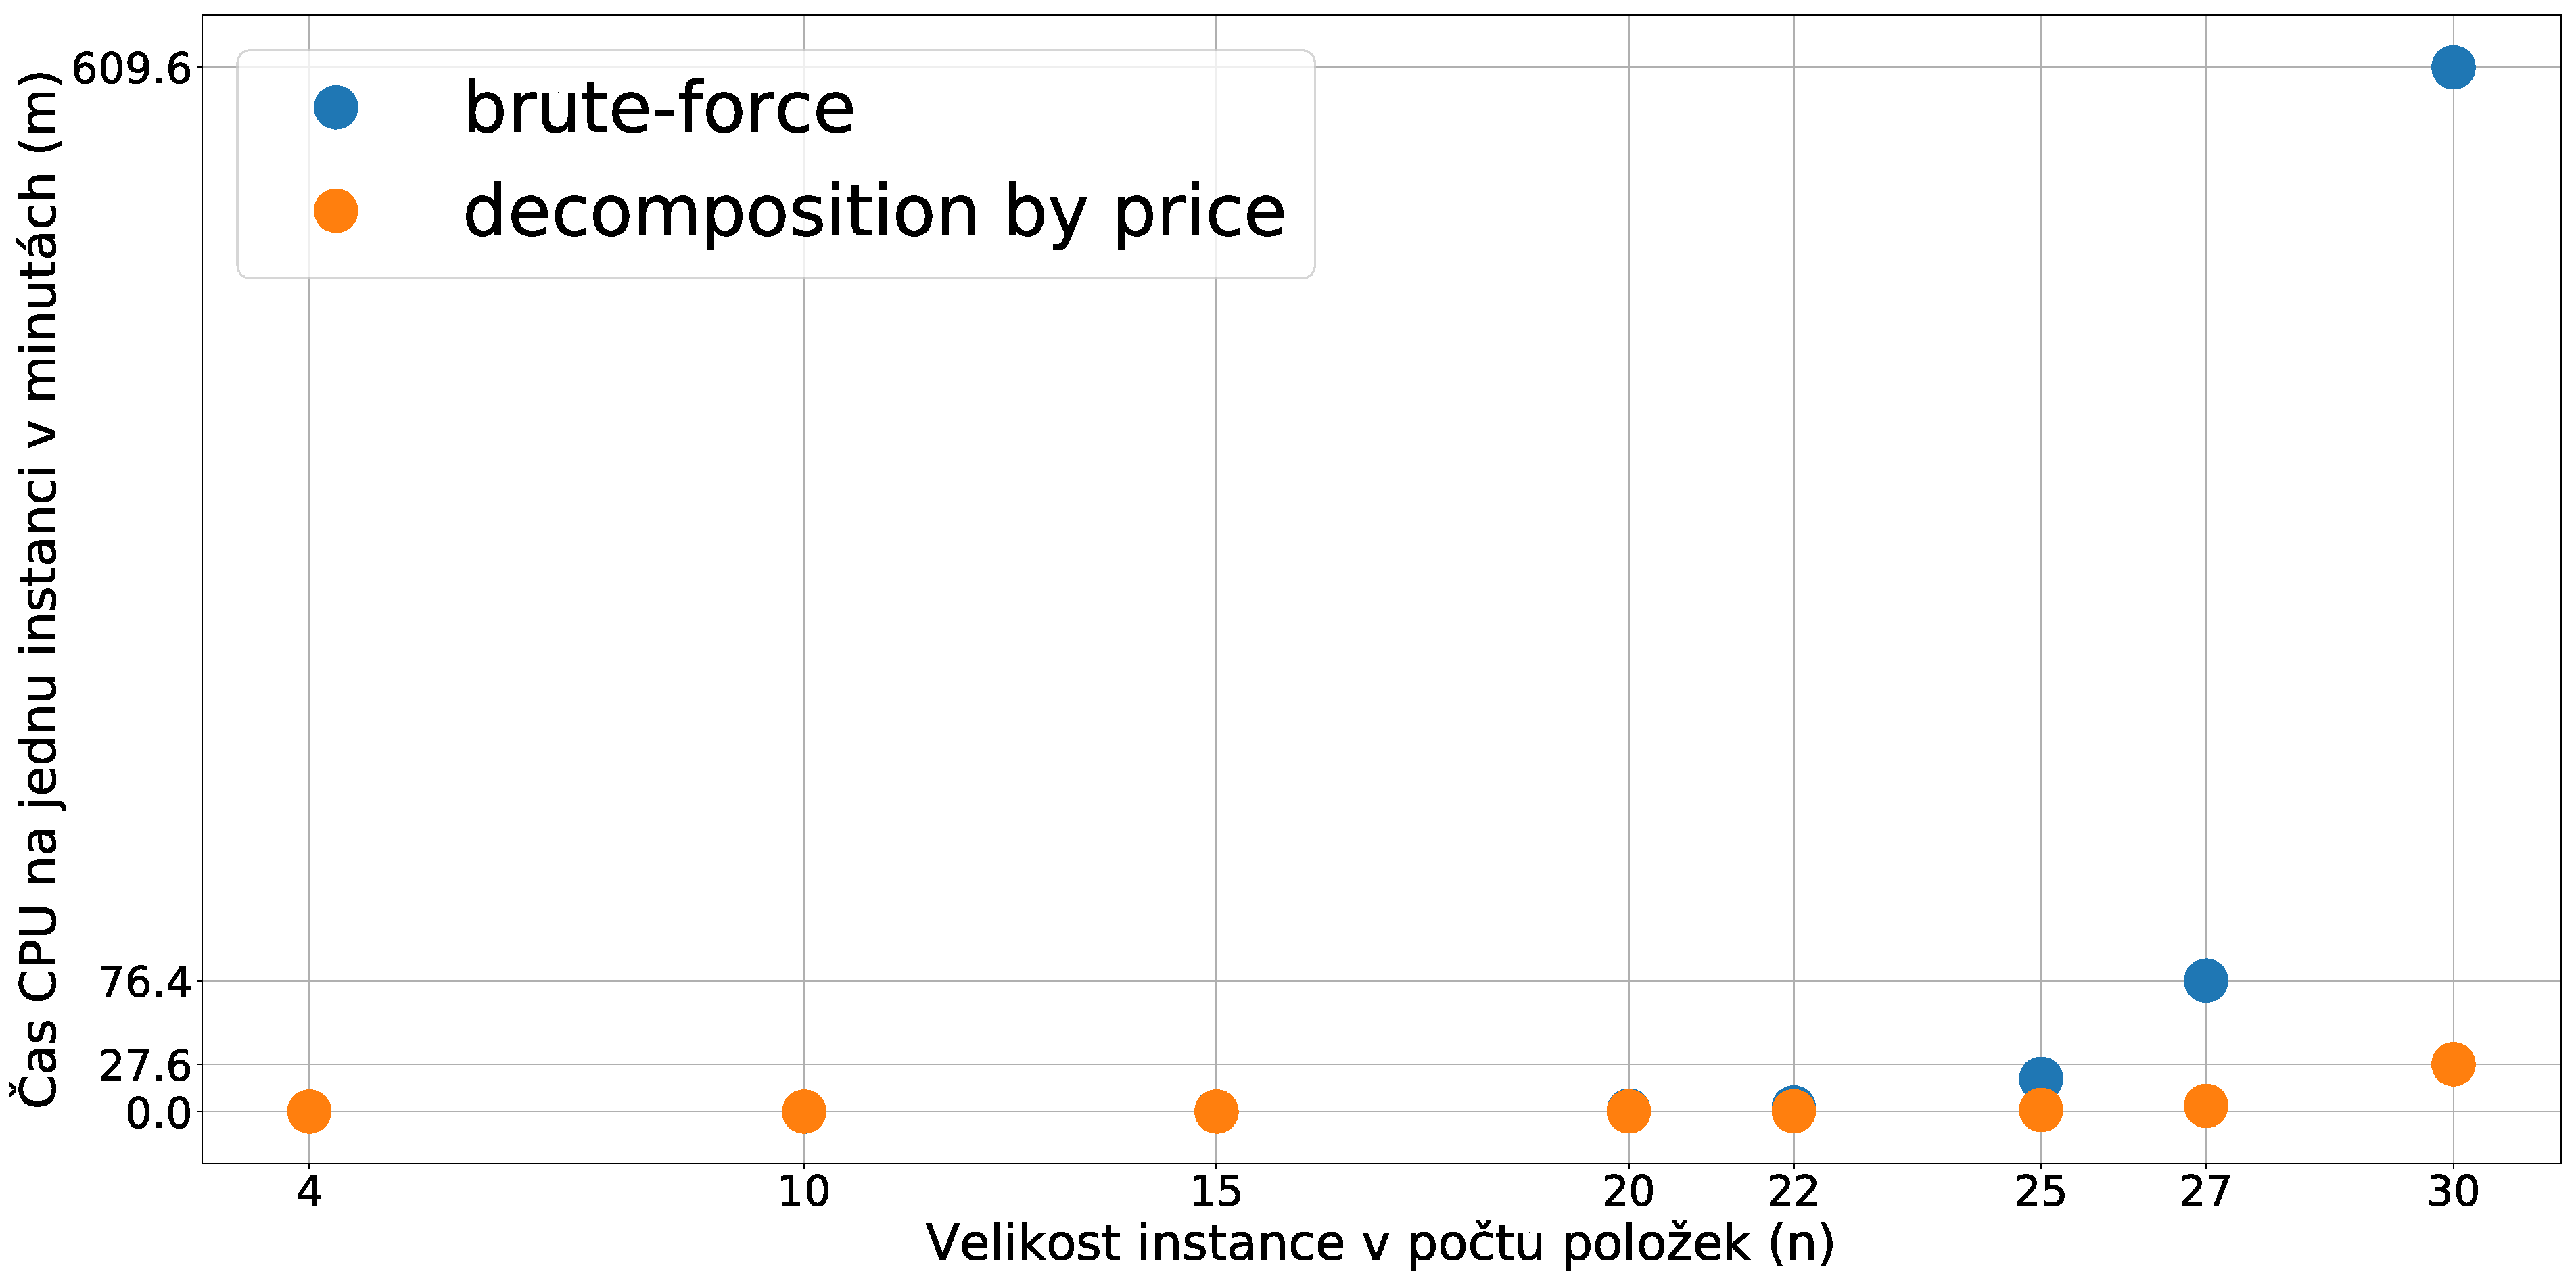
\includegraphics[scale=0.2]{img/tBavg}
 	\caption[1]{Brute-force ve srovnání s dynamickým programováním s dekompozicí podle ceny. Časová náročnost. Na grafu jsou průměrné hodnoty.}\label{fig:1}
 \end{figure} 	

\subsection{Srovnání exaktních metod pro řešení problému batohu}
Na grafu \ref{fig:1} jsem zanesl kromě brute-force řešení také řešení dekompozicí podle ceny. Je patrné, že složitost řešení s roustoucím $n$ pro brute-force metodu roste velice rychle,tedy řešení pomocí dynamického programování umožní velice uspořit čas. 


\begin{figure}[h]\centering
	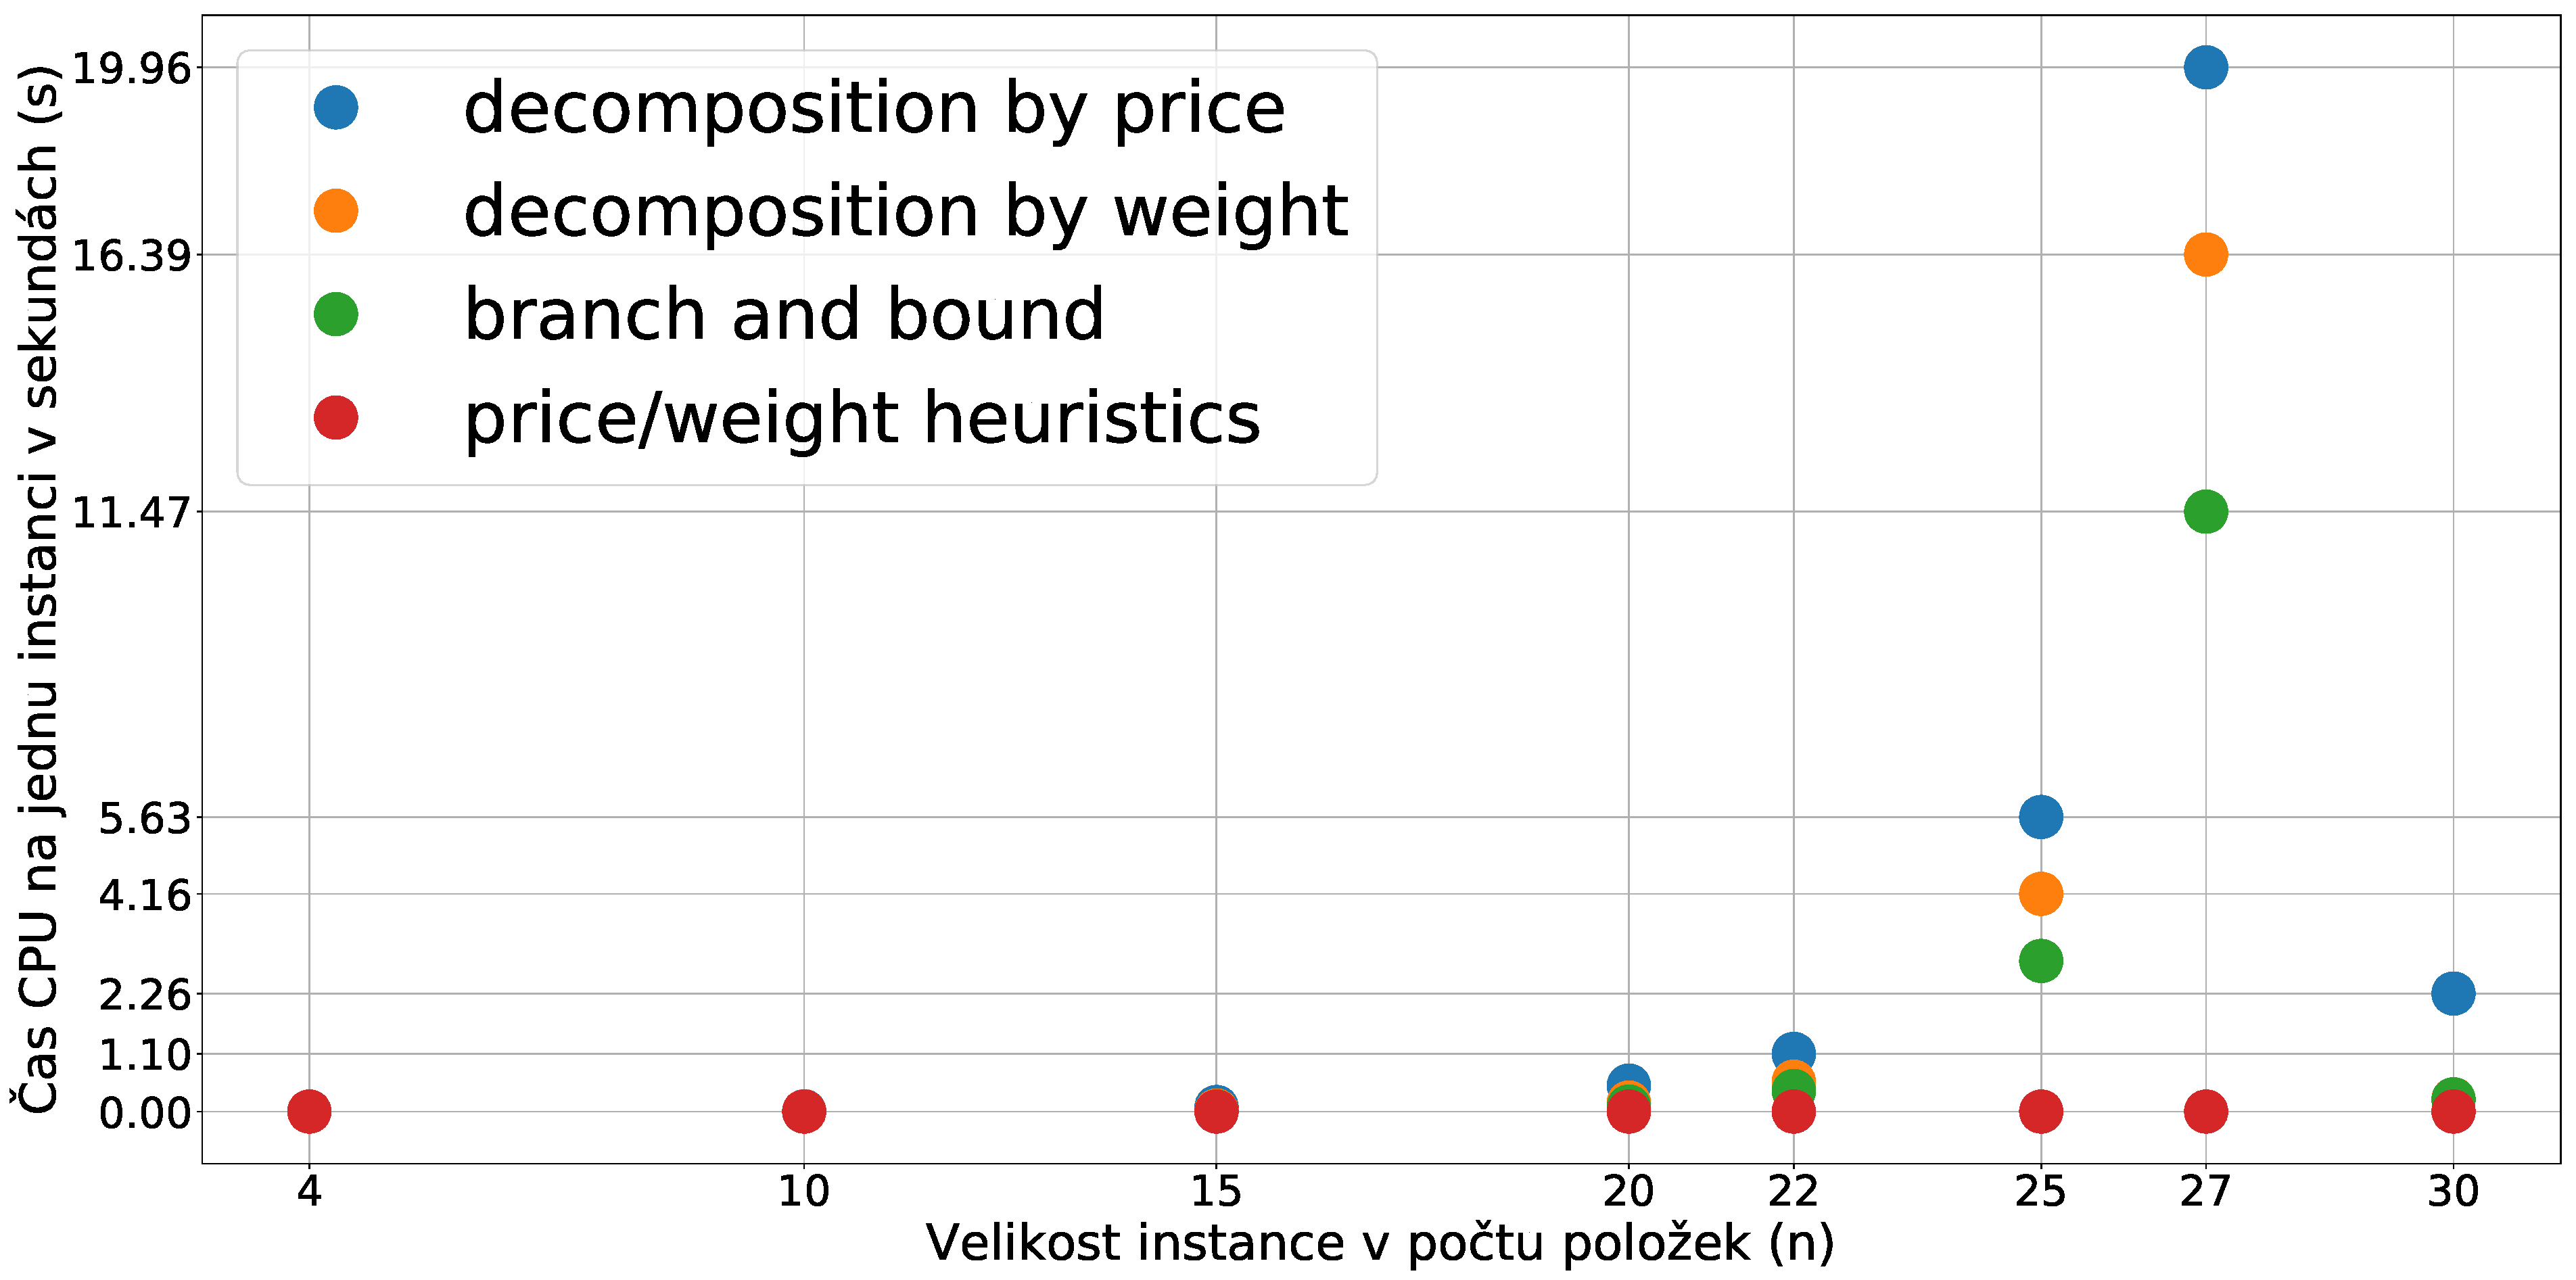
\includegraphics[scale=0.2]{img/tDavg}
 	\caption[2]{Časová náročnost obou způsobů dynamického programování, metody branch and bound a jednoduché heuristiky z předchozího úkolu. Na grafu jsou průměrné hodnoty.}\label{fig:2}
 \end{figure} 	
 

Na dalším grafu \ref{fig:2} jsem do grafu zanesl obě dekompozice, metodu větví a hranic a také heuristiku cena/hmotnost pro srovnání. 
U těchto metod mě velice zajímalo jaká je variance řešení. Pří porovnání průměrů a mediánu, byl v datech velký rozdíl. Z tohoto důvodu jsme se rozhodl vytvořit krabicové grafy (box ploty). Grafy zobrazují data podle kvartilů. Střední část je ohraničená 1. a 3. kvartilem. Jednotlivé body jsou odlehlé hodnoty. Celkově lze z box plotů vyčíst variabilitu dat. 

Všechny boxploty jsou vytvořeny s logaritmickým časem pro lepší vizualizaci, který však nemá vliv na variabilitu dat.

Na grafu \ref{fig:4} je vidět box plot vytvořený pro časy brute-force řešení. Je vidět, že výsledné hodnoty jsou blízko u sebe, tedy očekávaná je i nízka variance při výpočtu na různých instancí dat. 

\begin{figure}[h]\centering
	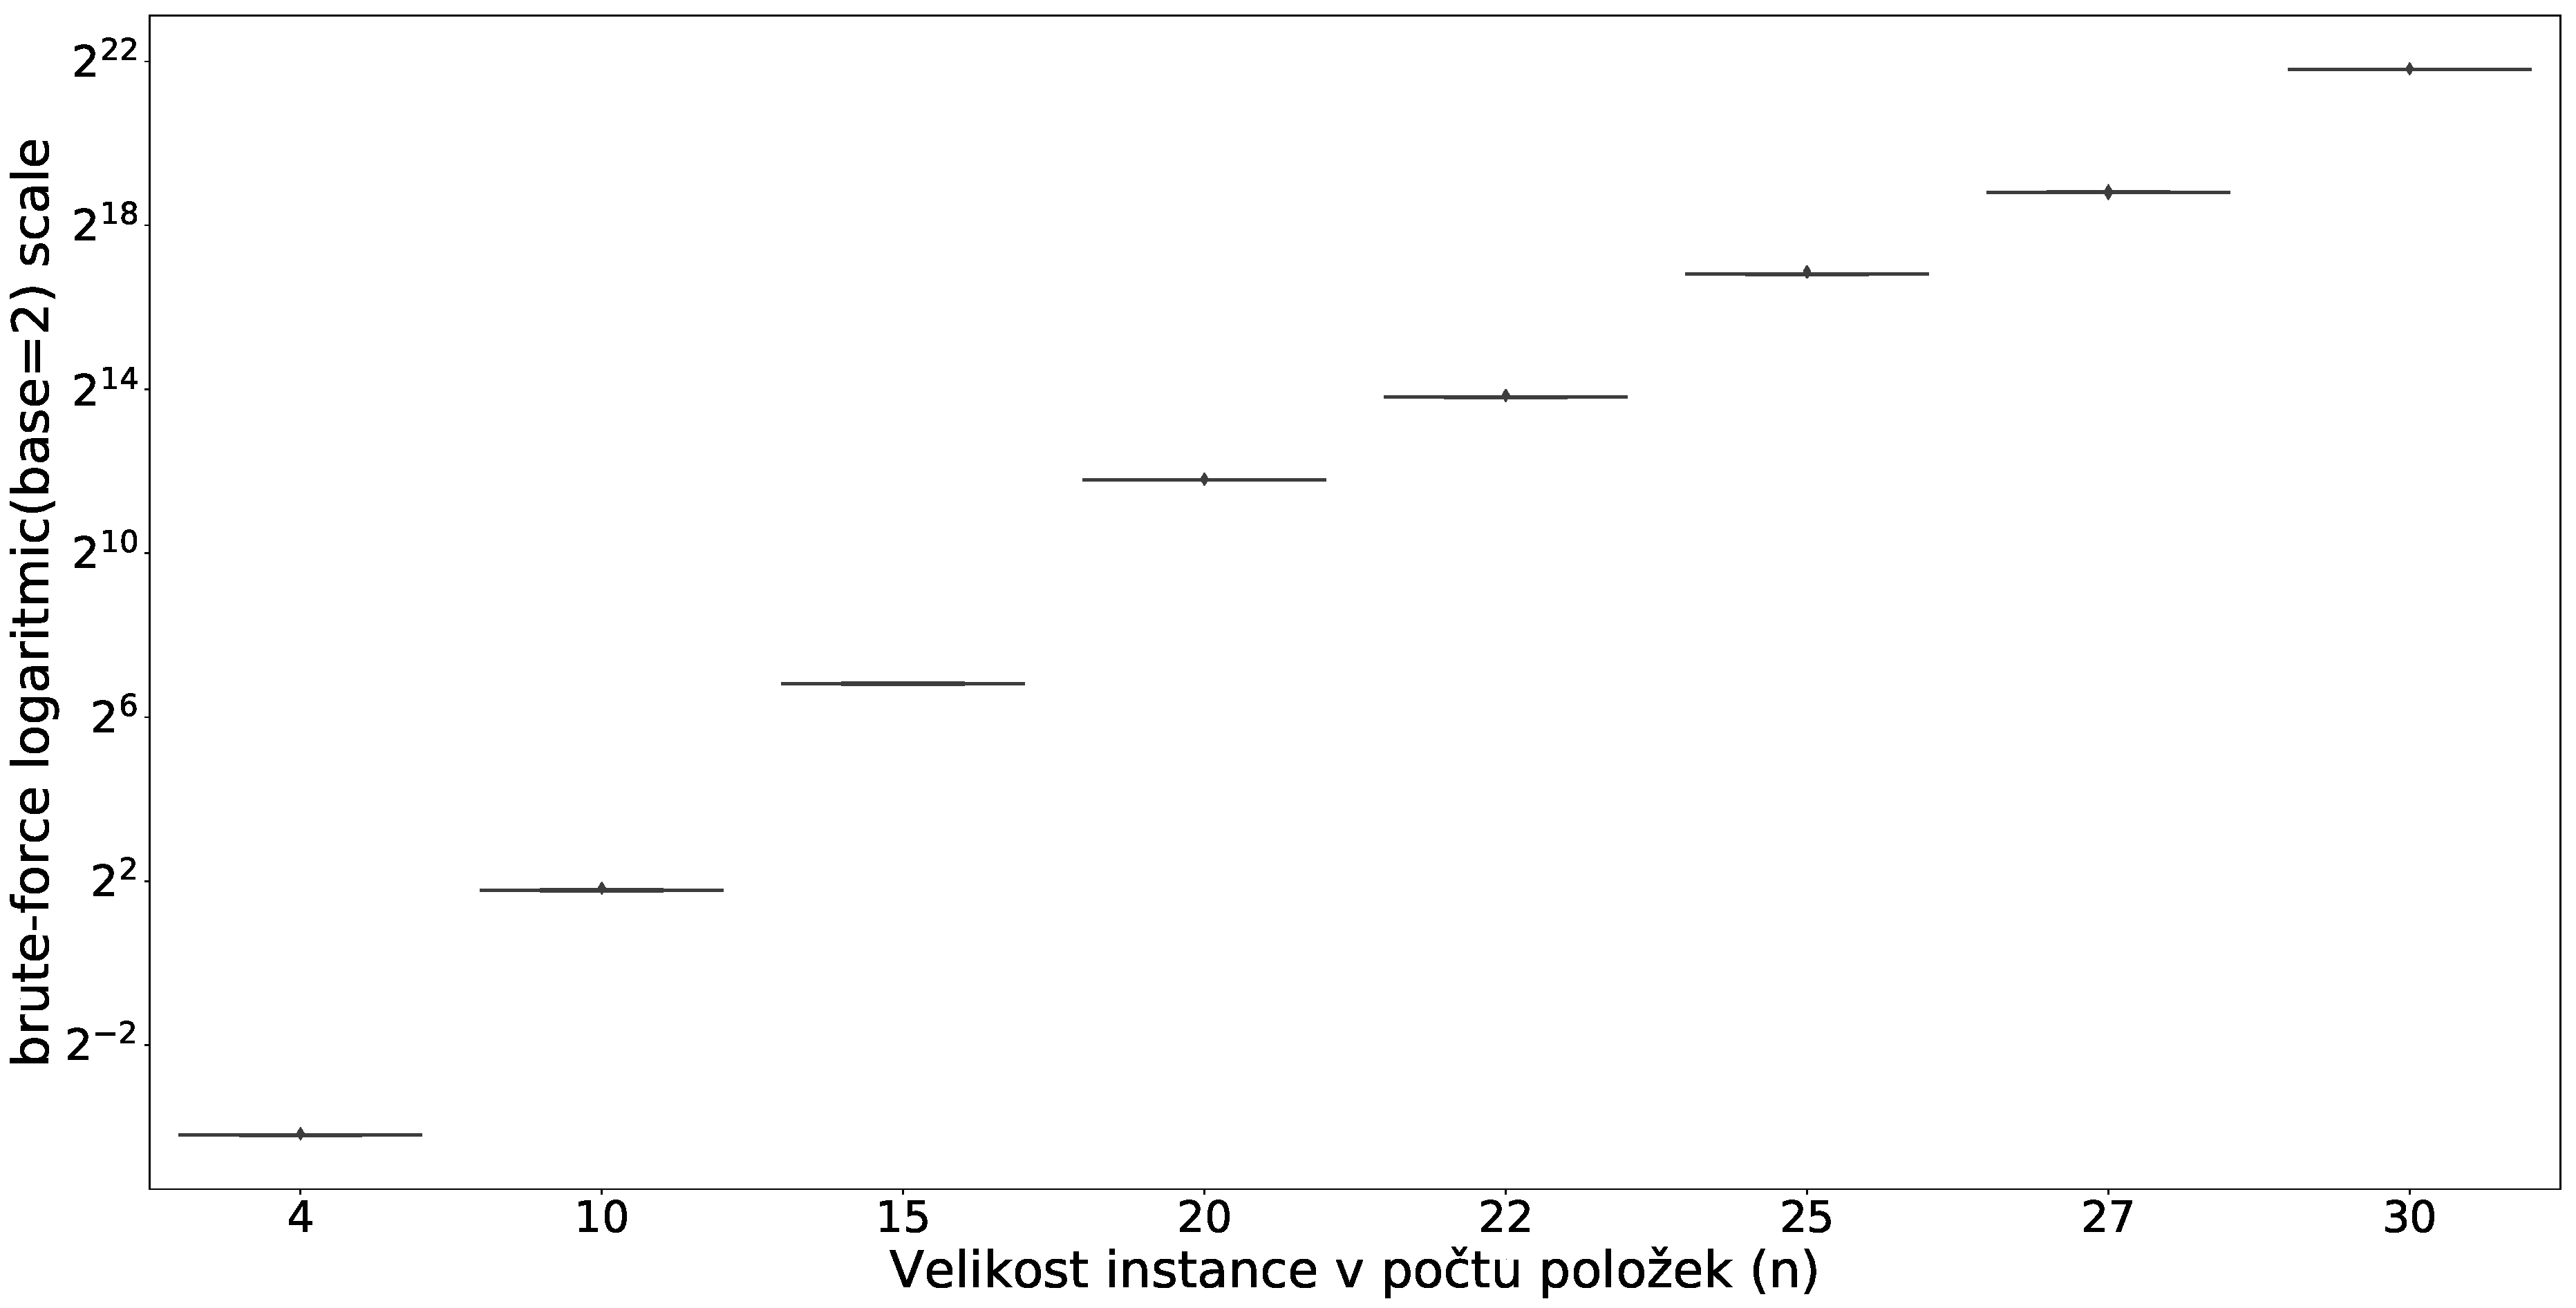
\includegraphics[scale=0.2]{img/boxB}
 	\caption[2]{Krabicový graf popisující variabilitu měření metody hrubé síly vždy pro 50 instancí problému.}\label{fig:4}
 \end{figure} 		

Další dva grafy \ref{fig:5} a \ref{fig:6} jsou výsledky z měření dynamického programování. Jak pro dekompozici podle ceny, tak i podle kapacity. Na tomto grafu jsou zajímavé body, které jsou vidět nad jednotlivými boxy. Tyto odlehlé hodnoty jsou "těžké" instance problému, pro které trval výpočet dlouho oproti obvyklé době. Je vidět, že výpočet na těchno instancích trvá velmi dlouho. Dalšími měřeními by bylo zajímavé zjistit, jaké specifikace má problém, který je pro dekompozici složitý.

\begin{figure}[h]\centering
	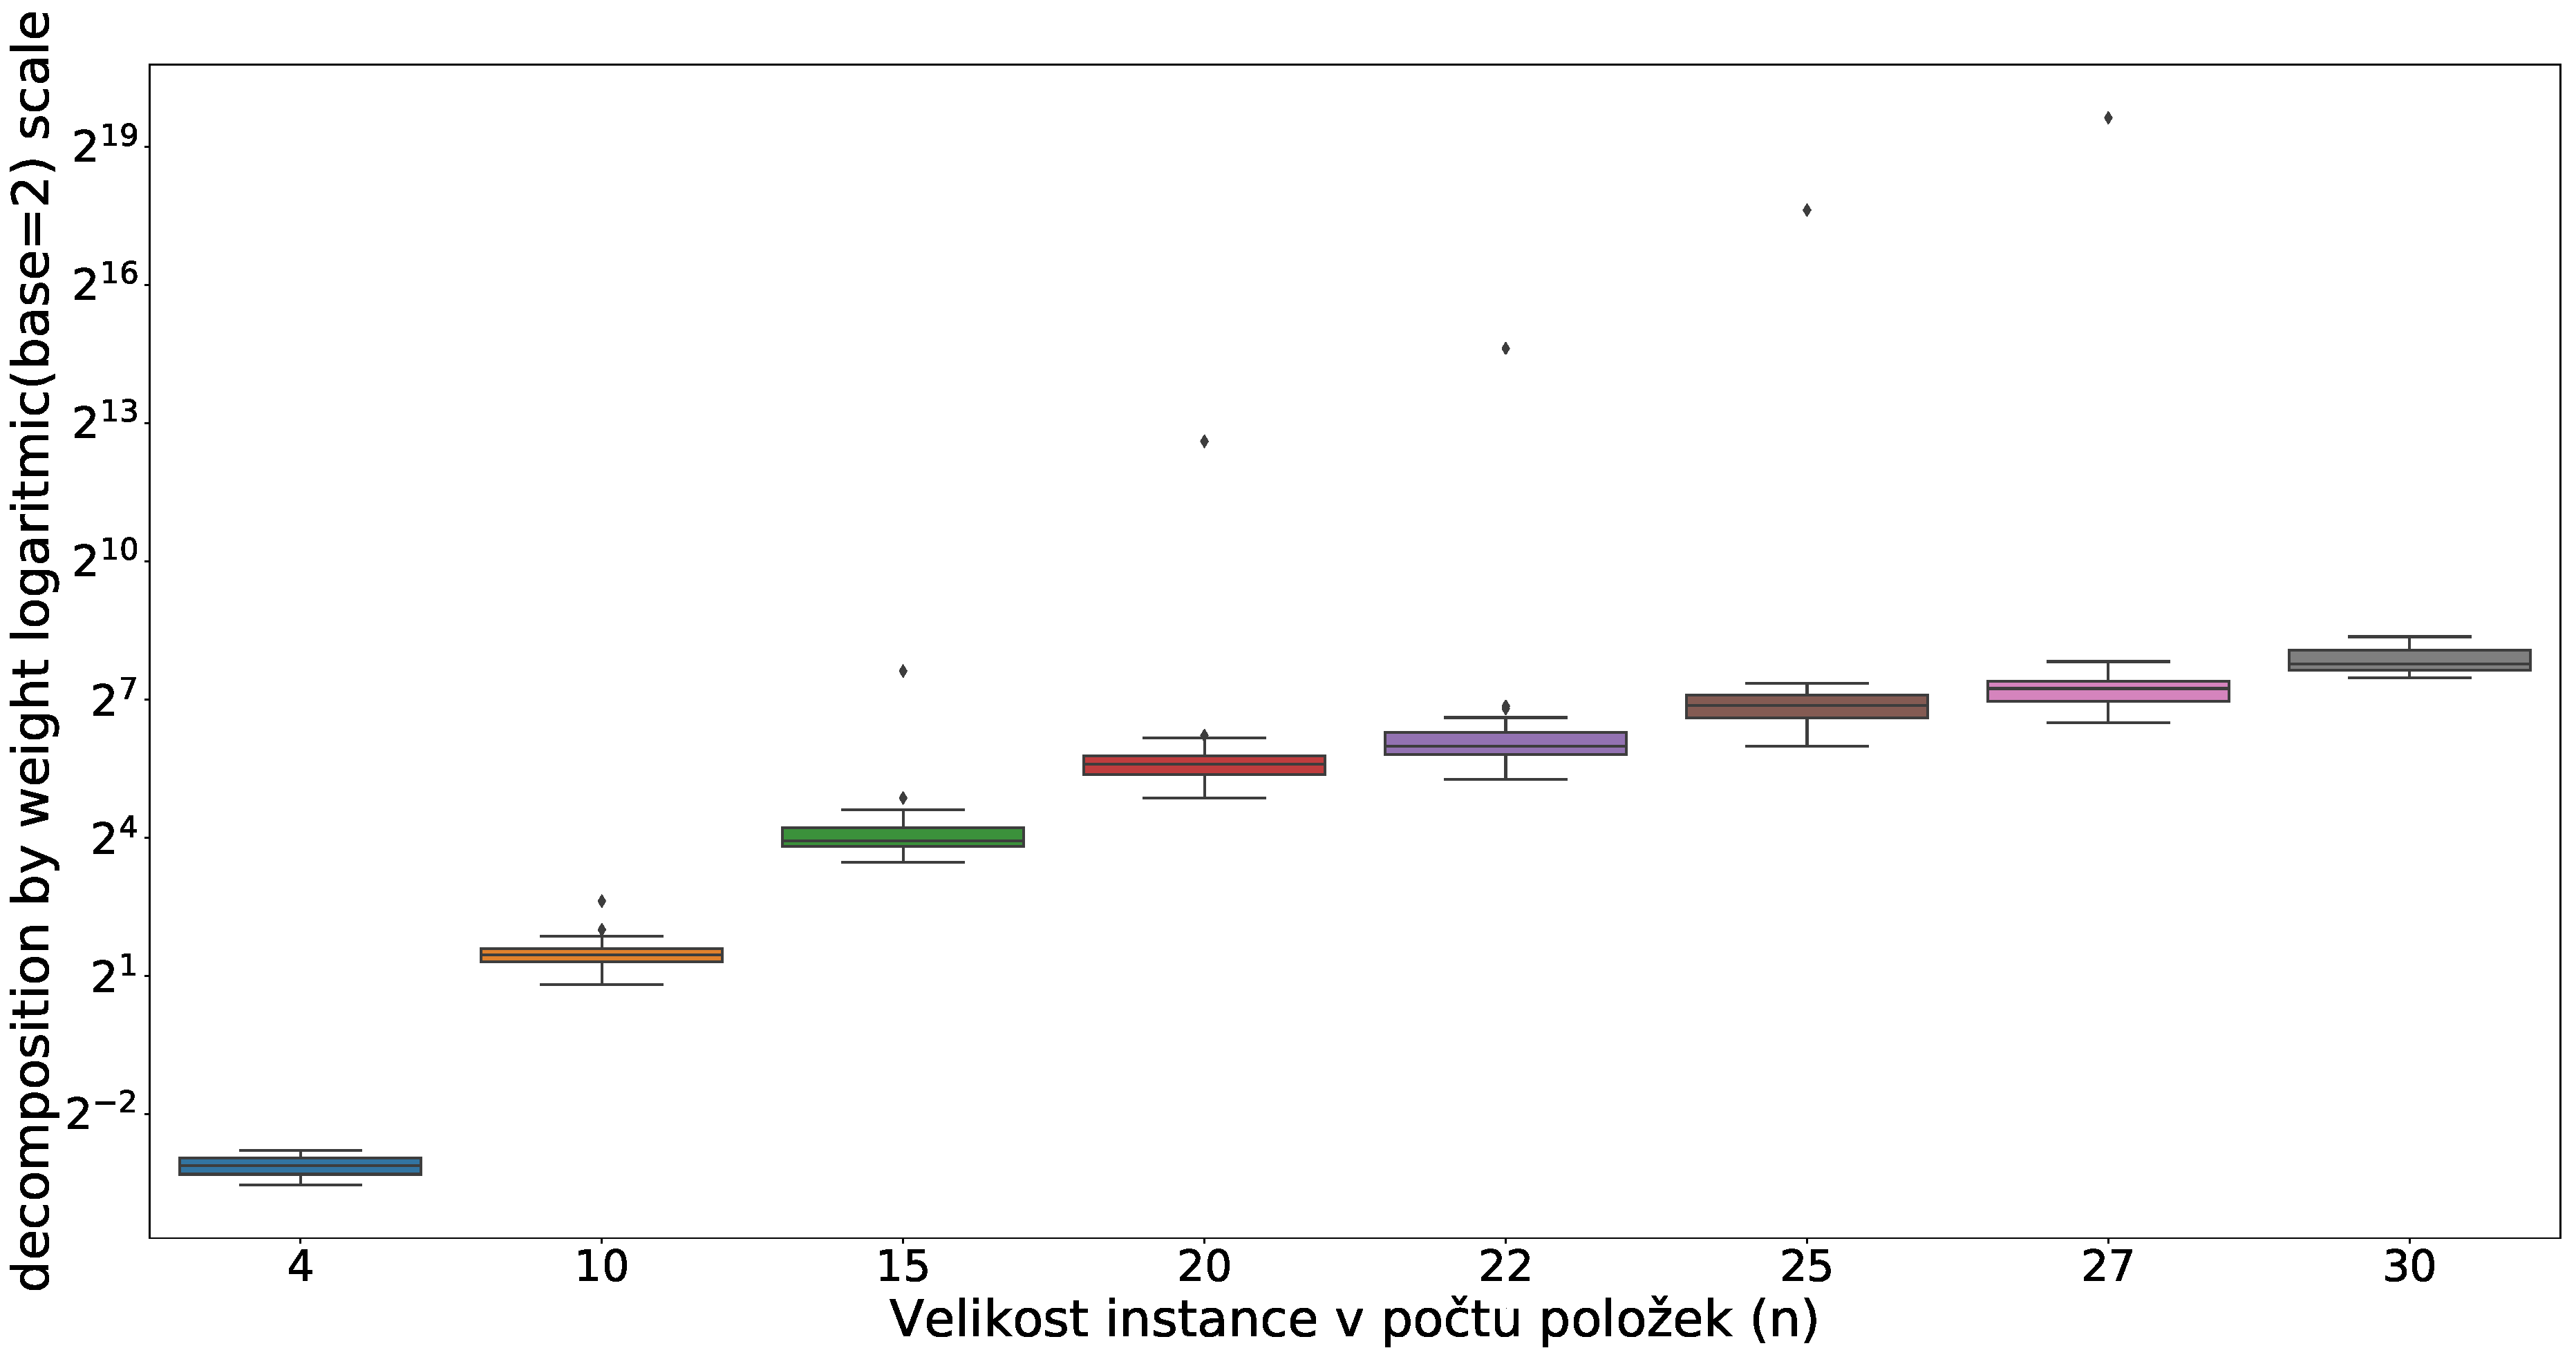
\includegraphics[scale=0.2]{img/boxDW}
 	\caption[2]{Krabicový graf popisující variabilitu měření metody dekompozice podle kapacity vždy pro 50 instancí problému.}\label{fig:5}
 \end{figure} 	
 \begin{figure}[h]\centering
	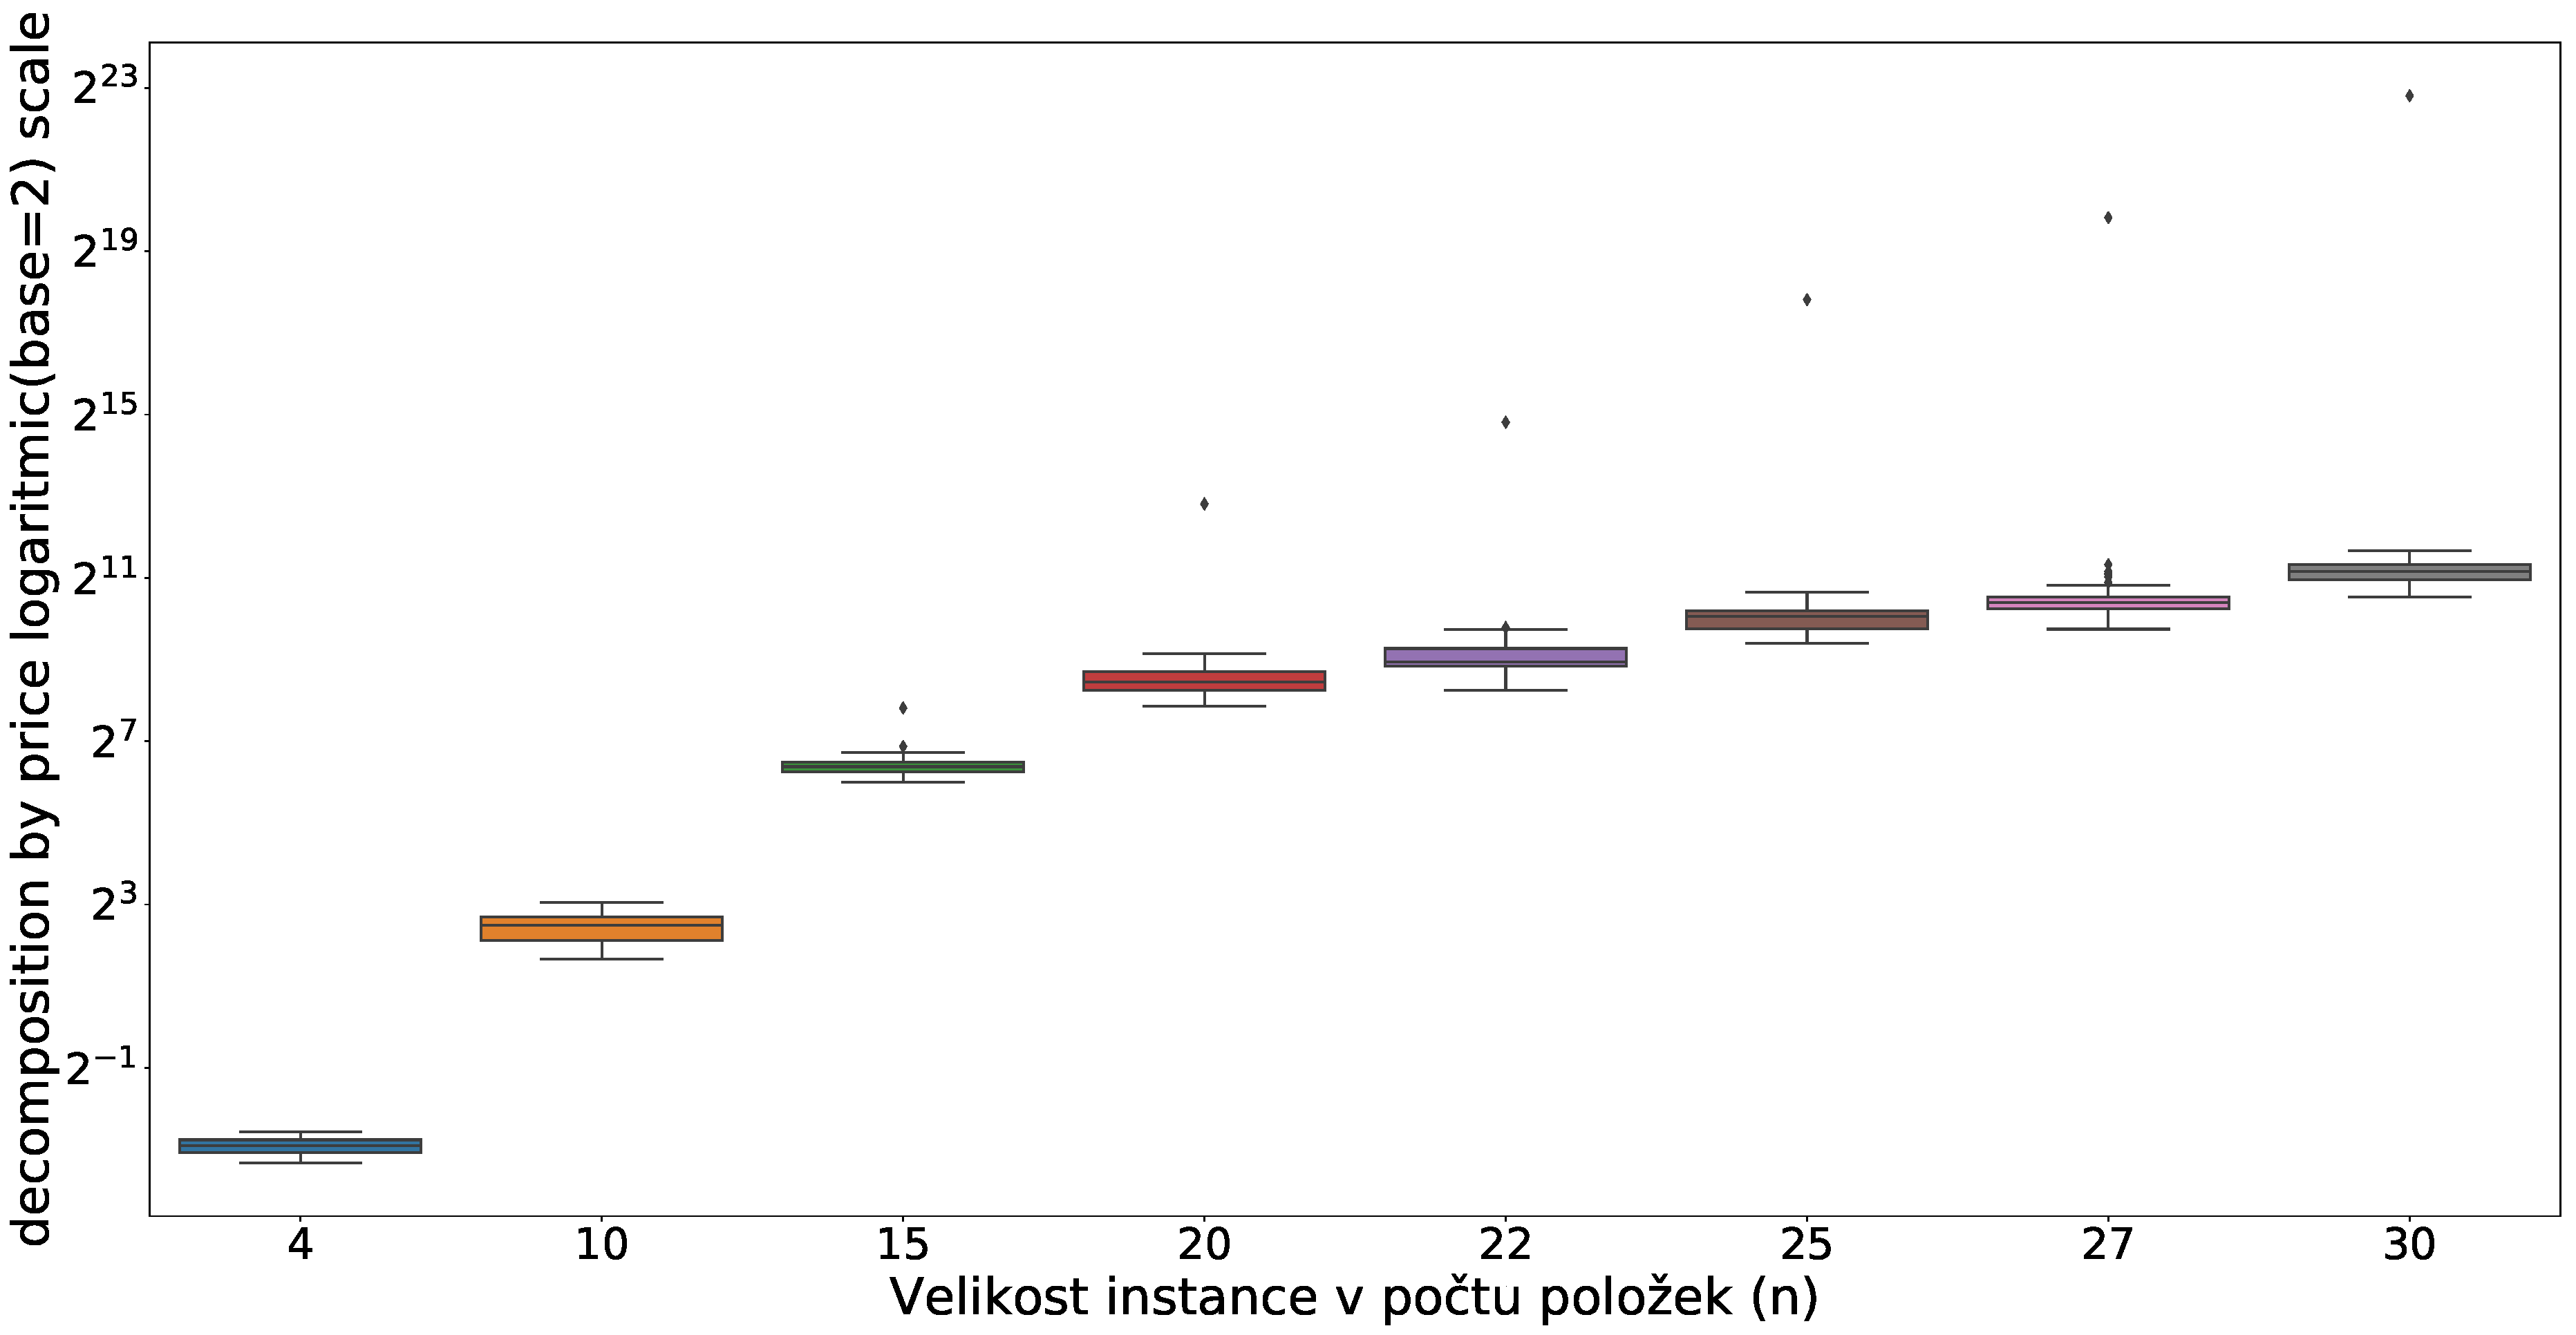
\includegraphics[scale=0.2]{img/boxDC}
 	\caption[2]{Krabicový graf popisující variabilitu měření metody dekompozice podle ceny vždy pro 50 instancí problému.}\label{fig:6}
 \end{figure}

Na grafu \ref{fig:7} je vidět boxplot pro metodu větví a hranic. I zde se nacházejí těžké instance problému. Dále je z grafu patná větší variance časů řešení, kde pro nějaké problémy je metoda velice rychlá, ale existuje mnoho instancí, ve kterých nedojde k požadovanému prořezání. Opět by bylo zajímavé najít tyto optížné instance a nebo je umět například generovat.

I přes horší časy při experimentech má dynamického programování výhodu, že má mnohem menší varianci výpočetních časů.

\begin{figure}[h]\centering
	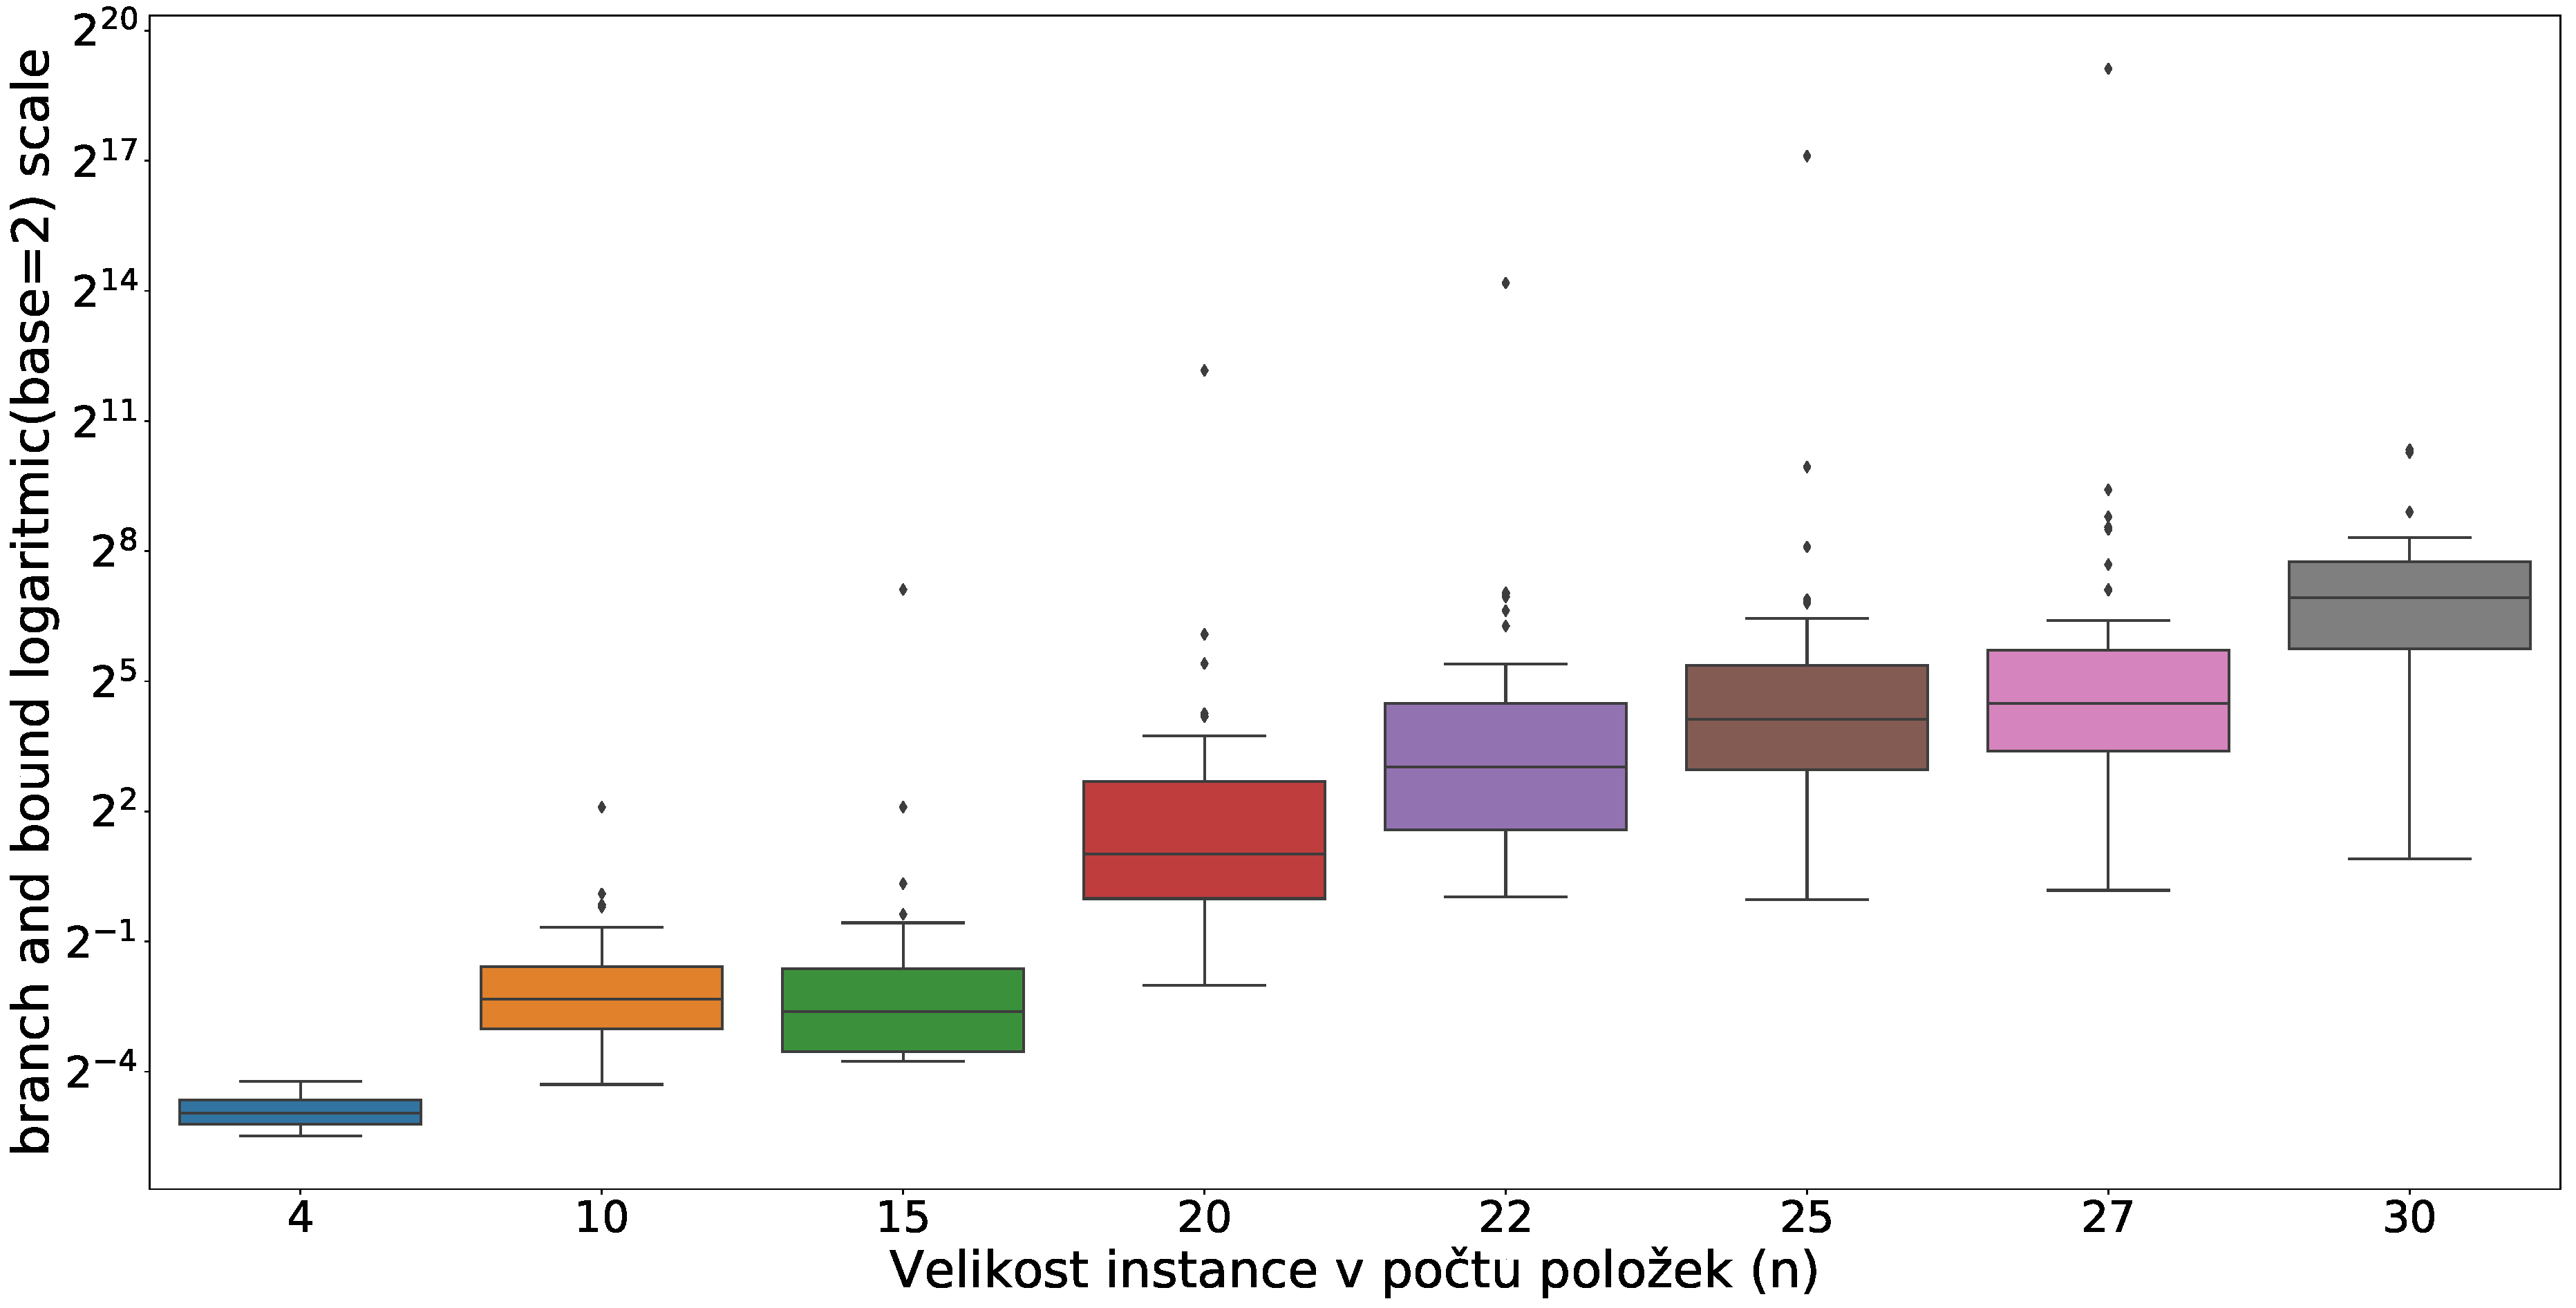
\includegraphics[scale=0.2]{img/boxBB}
 	\caption[2]{Krabicový graf popisující variabilitu měření metody větví a hranic vždy pro 50 instancí problému.}\label{fig:7}
 \end{figure} 	

\subsection{FPTAS meření času}

FPTAS jsem otestoval s různými nastaveními pro maximální povolenou chybu. Zde jsem časové grafy uvedl jak pro průměr, tak pro medián, po předchozím pozorování na krabicových grafech. Je vidět, že výsledný čas se přesně odvíjí od nastavené chyby. Velkou výhodou algoritmu je tedy možost nastavení maximální chyby.

Na grafech \ref{fig:8} a \ref{fig:9} jsou vidět výsledky měření pro různá $\epsilon$ a do grafu byly pro srovnání přidány metody dekompozice podle ceny a metoda větví a hranic. Je vidět, že změnou parametru lze jednoduše měnit výpočetní náročnost.

 \begin{figure}[h]\centering
	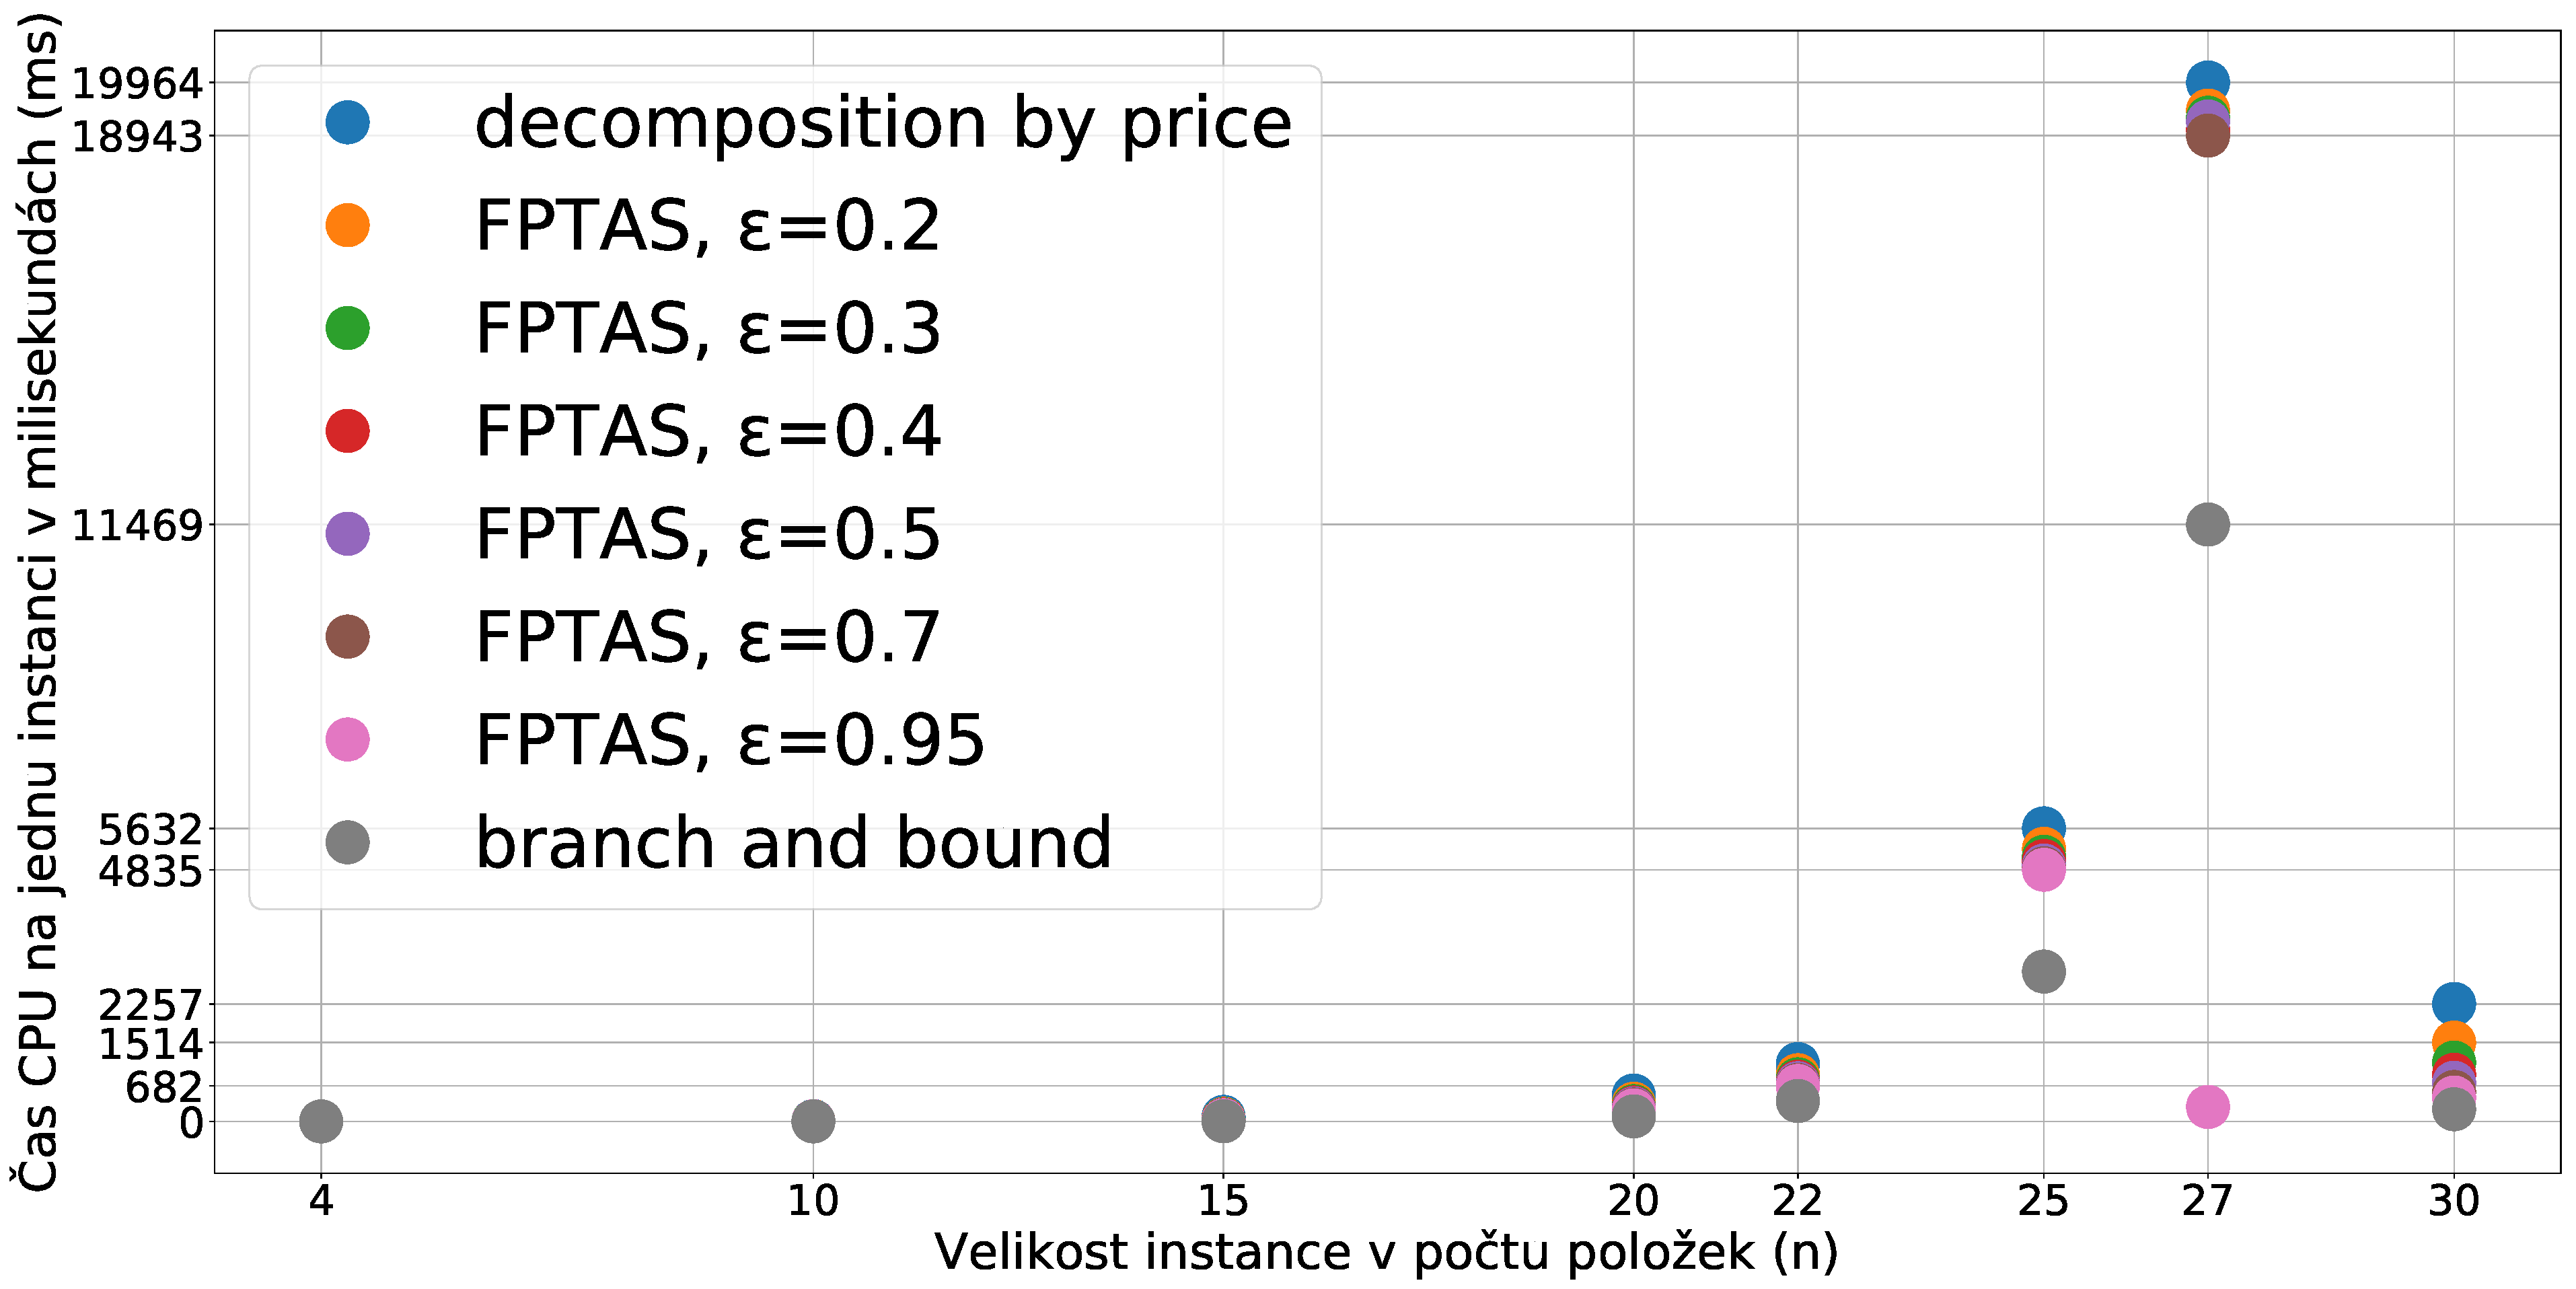
\includegraphics[scale=0.2]{img/FPTASavg}
 	\caption[2]{Časová náročnost pro různé volby $\epsilon$ v FPTAS ve srovnání s dekompozicí a metodou branch and bound. Hodnoty jsou uvedeny pro průměr.}\label{fig:8}
 \end{figure} 	
 \begin{figure}[h]\centering
	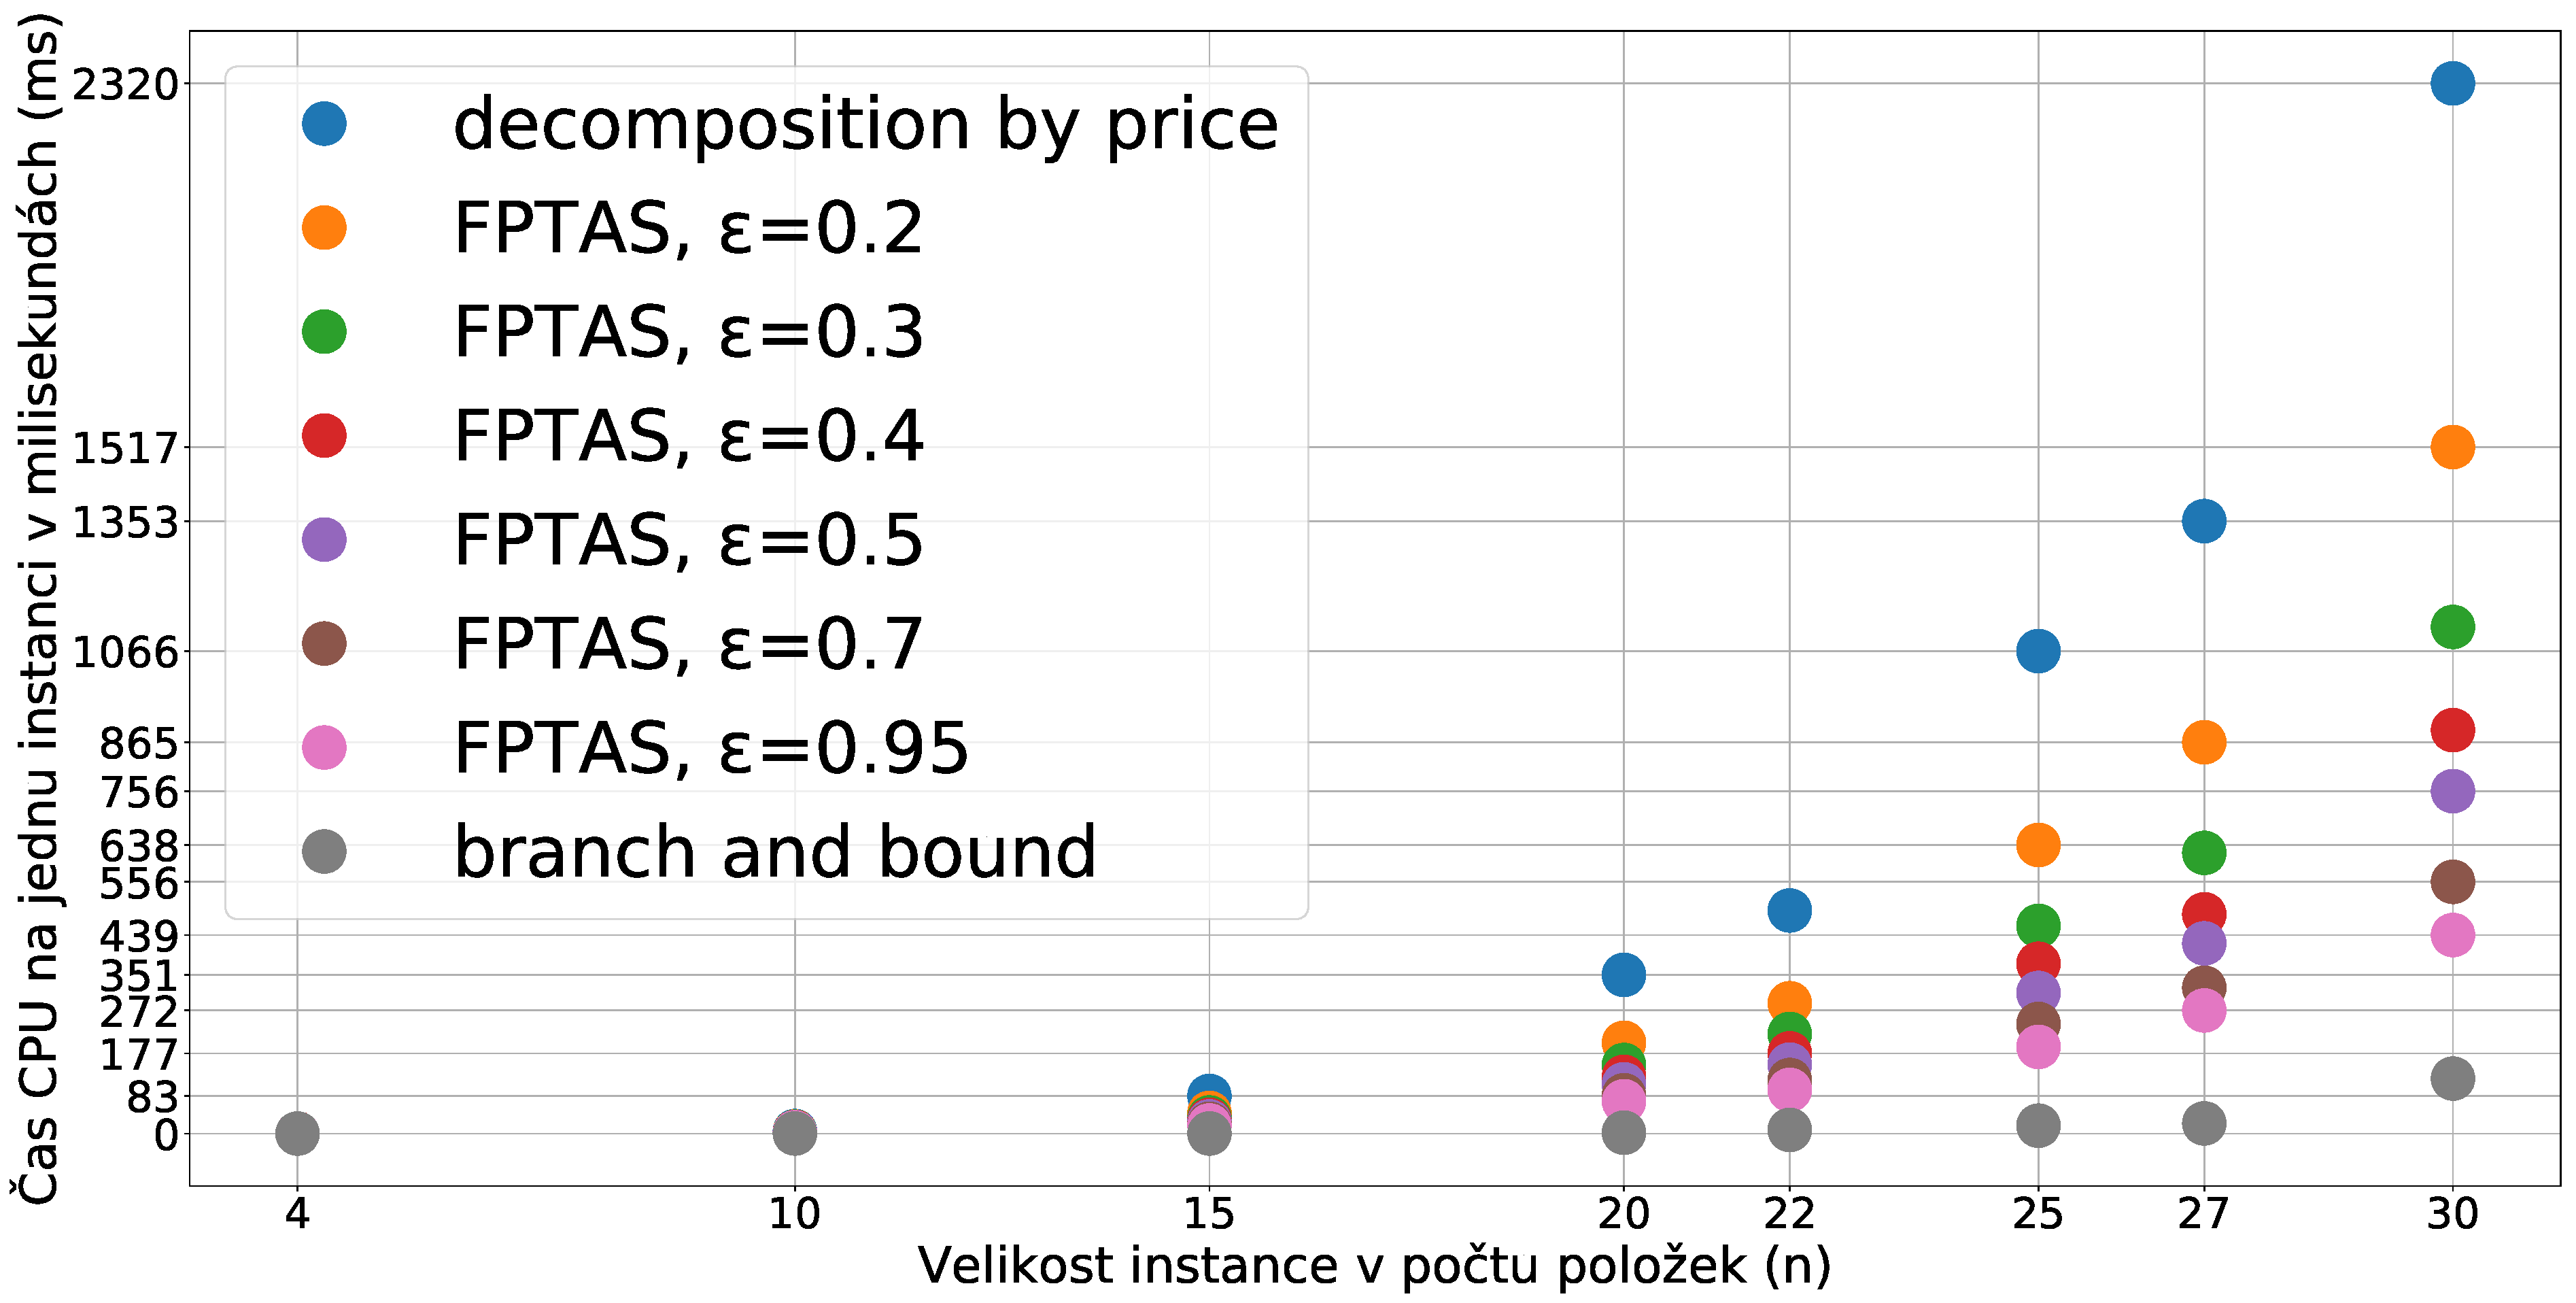
\includegraphics[scale=0.2]{img/FPTAS50}
 	\caption[2]{Časová náročnost pro různé volby $\epsilon$ v FPTAS ve srovnání s dekompozicí a metodou branch and bound. Hodnoty jsou uvedeny pro medián.}\label{fig:9}
 \end{figure} 	
 
Na těchto měření jsou také zajímavé krabicové grafy. Například pro $\epsilon=0.5$ na grafu \ref{fig:11} se zde stále vyskytují dané "těžké" problémy. Ale při volbě $\epsilon=0.95$ na grafu \ref{fig:10} se již pro $n=27$ daný problém nevyskytuje a tento skok bude patrný i na grafu závislosti $\epsilon$ a času. Tedy aproximační schéma dokázalo problém dostatečně zjednodušit pro rychlé řešení avšak na úkor negarantování nějaké přiměřené hranice chyby. Toto je nejvíce patrné pro $\epsilon=0.99$ na grafu \ref{fig:12}. V těchto případech nám však algoritmus již negarantuje přijatelnou relativní chybu.
 
 \begin{figure}[h]\centering
	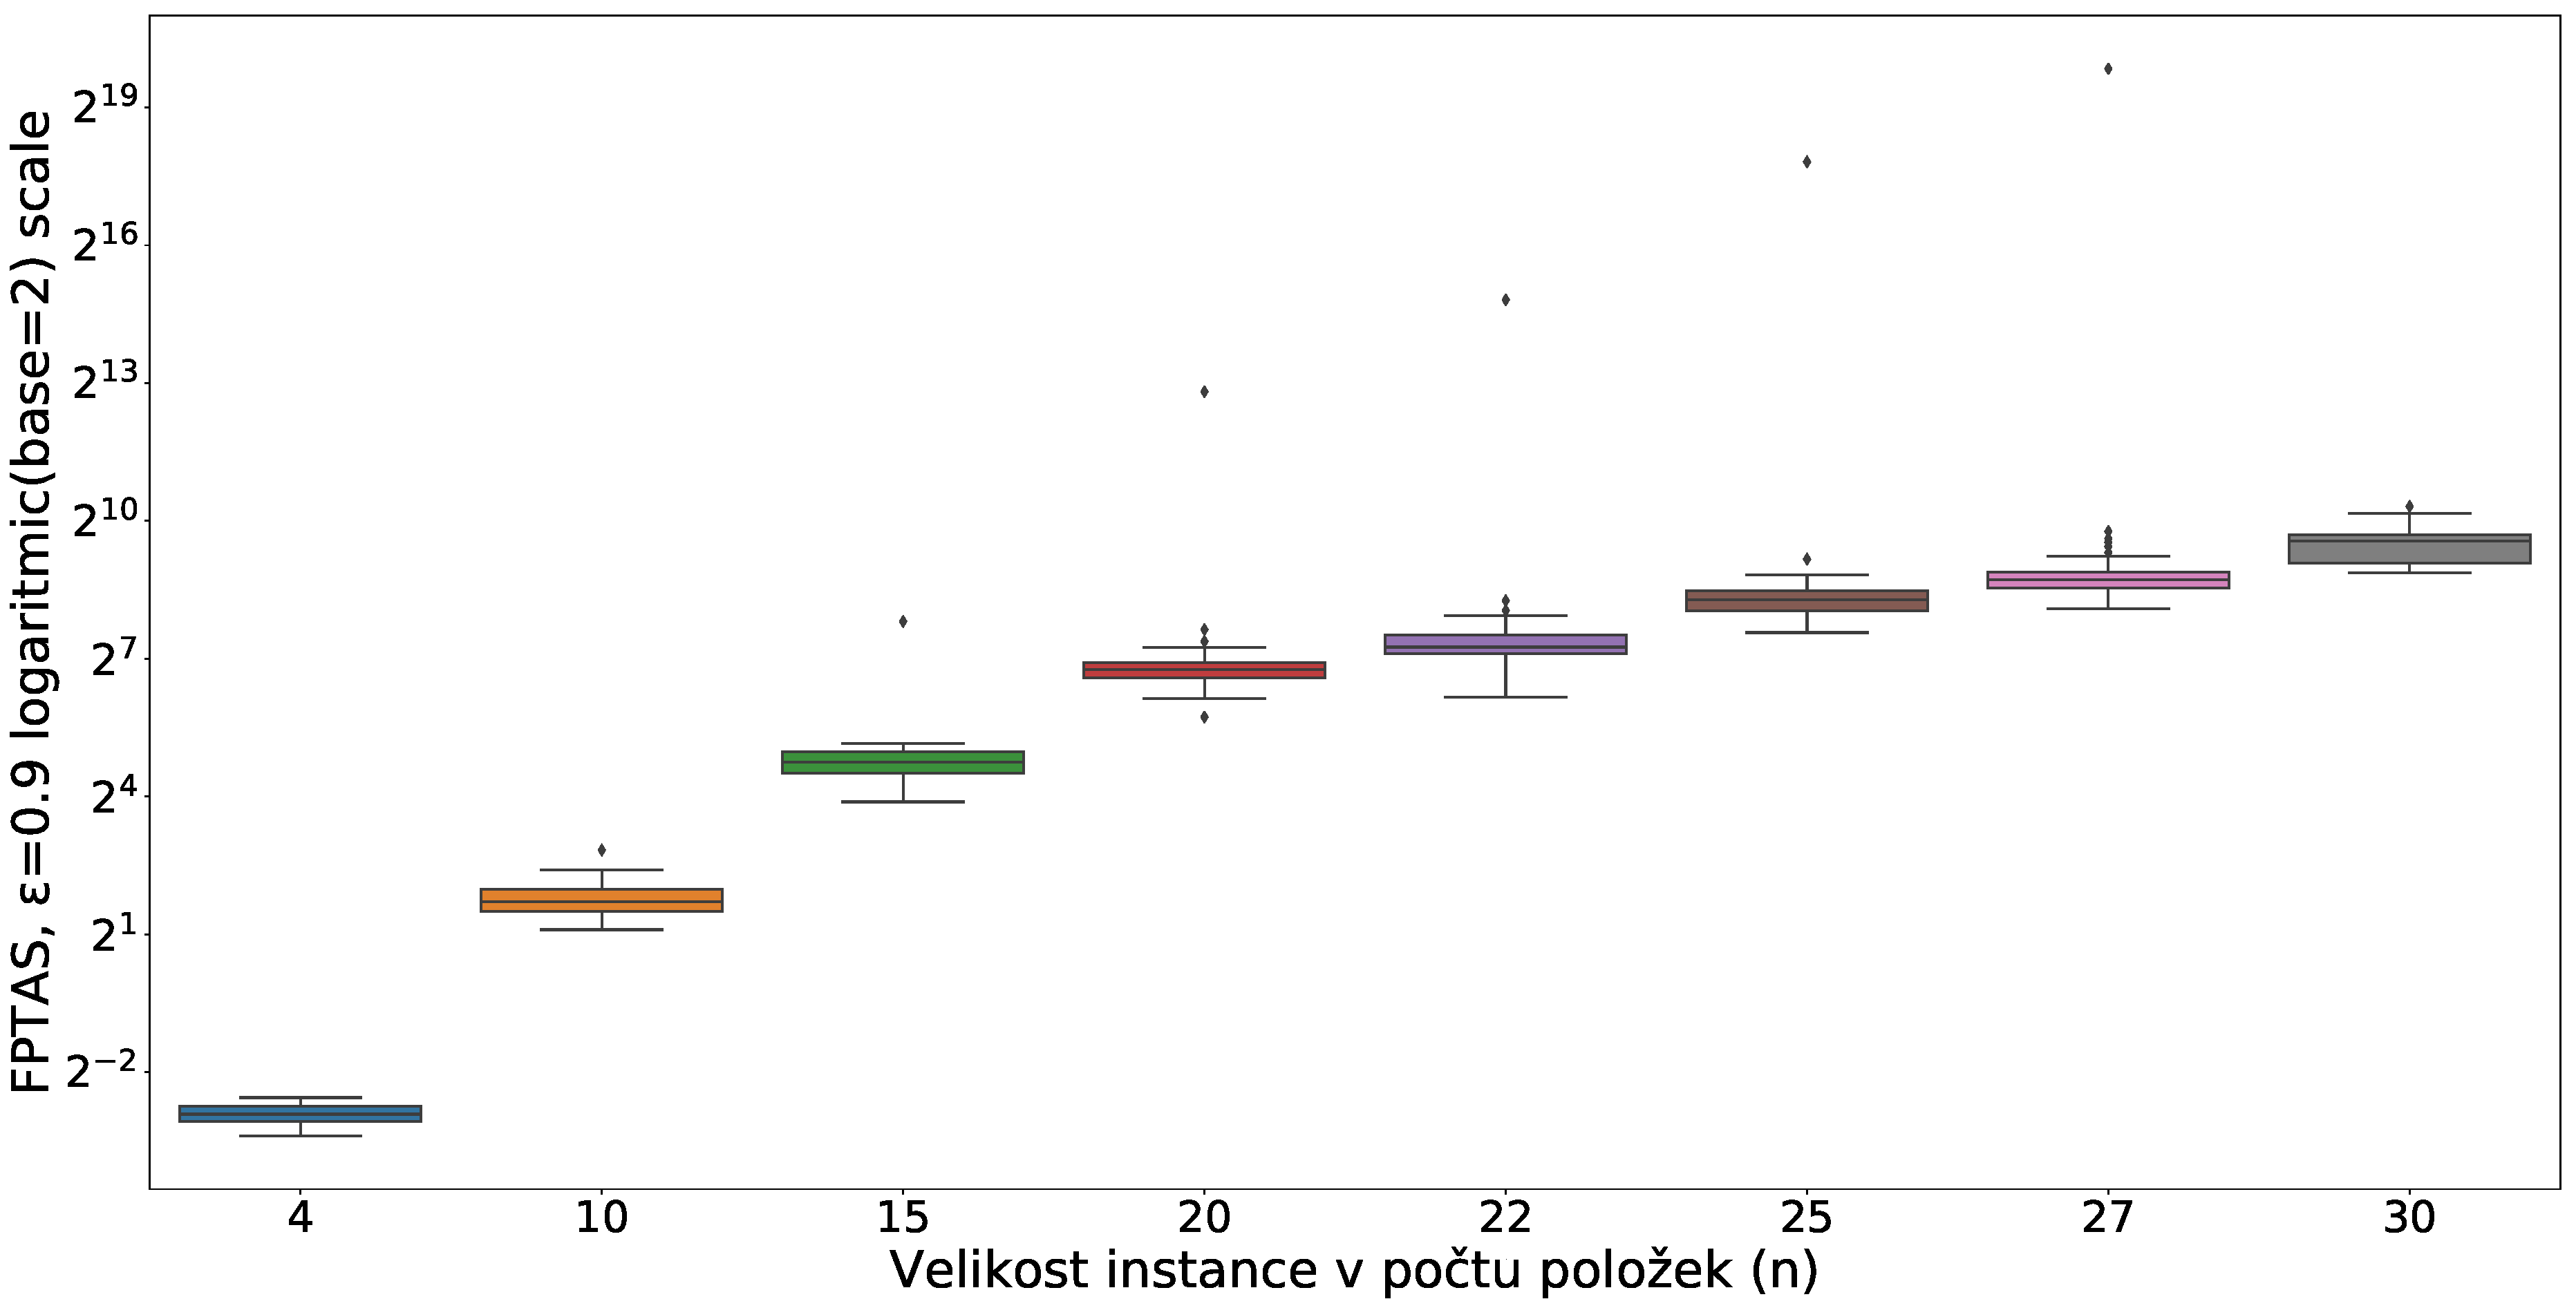
\includegraphics[scale=0.2]{img/boxF50}
 	\caption[2]{Krabicový graf popisující variabilitu měření metody FPTAS $\epsilon = 0.5$ vždy pro 50 instancí problému.}\label{fig:11}
 \end{figure} 	
 \begin{figure}[h]\centering
	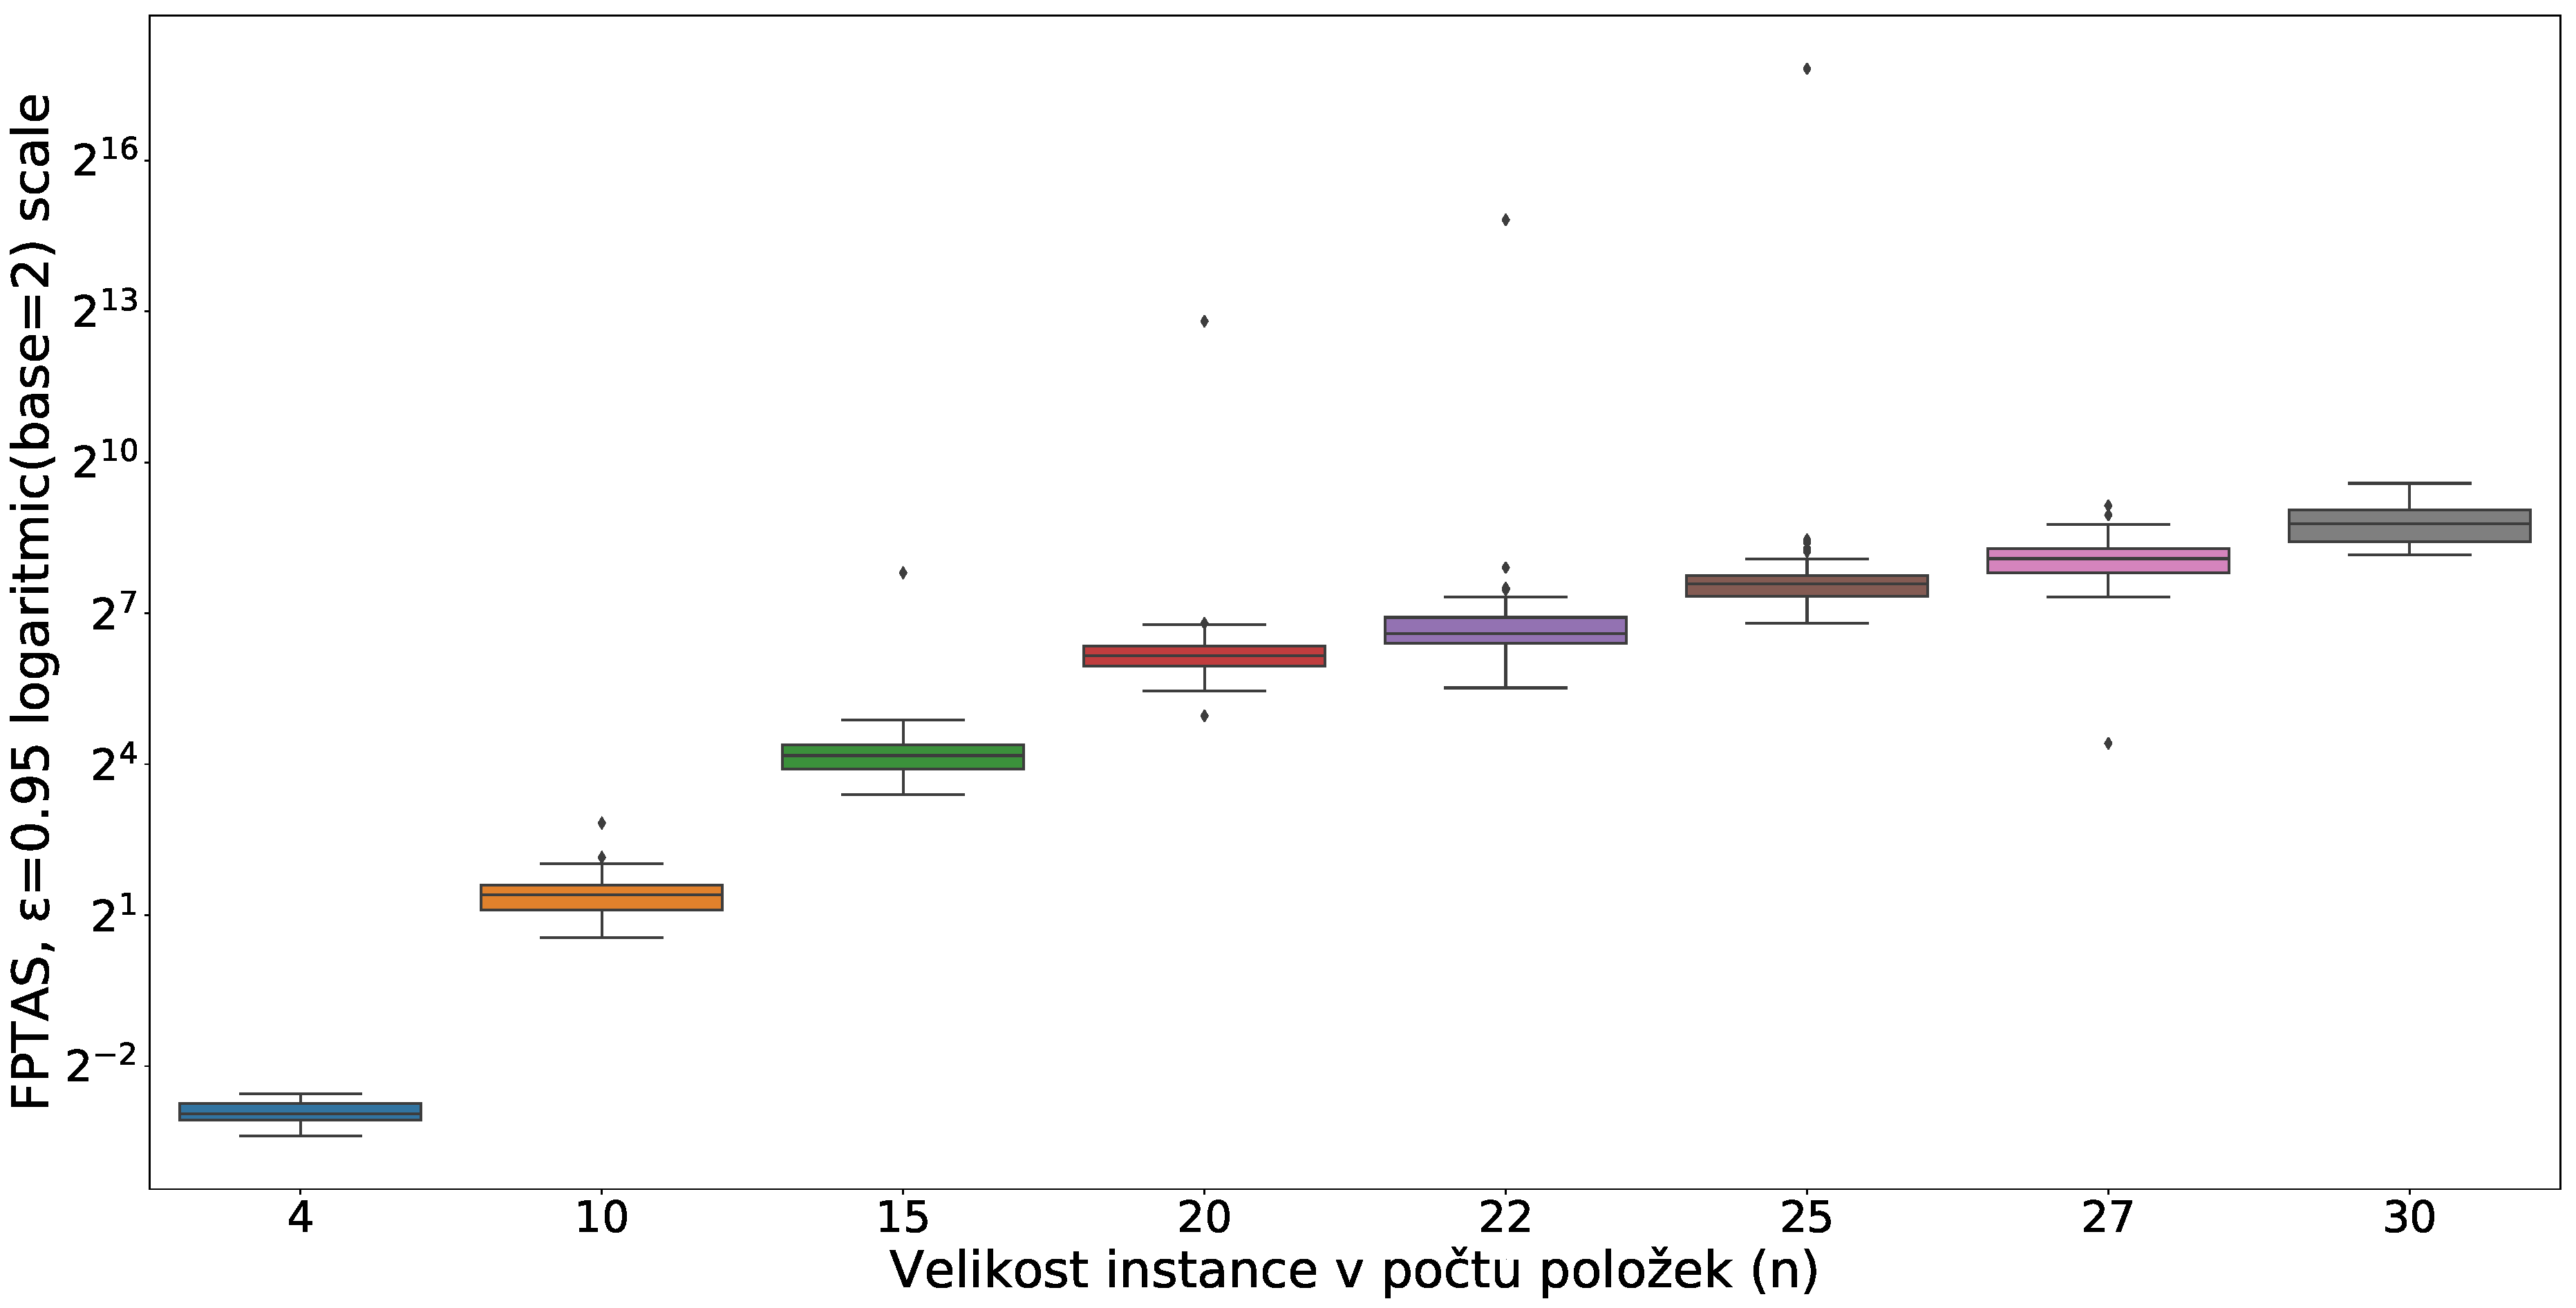
\includegraphics[scale=0.2]{img/boxF95}
 	\caption[2]{Krabicový graf popisující variabilitu měření metody FPTAS $\epsilon = 0.95$ vždy pro 50 instancí problému.}\label{fig:10}
 \end{figure} 	
 \begin{figure}[h]\centering
	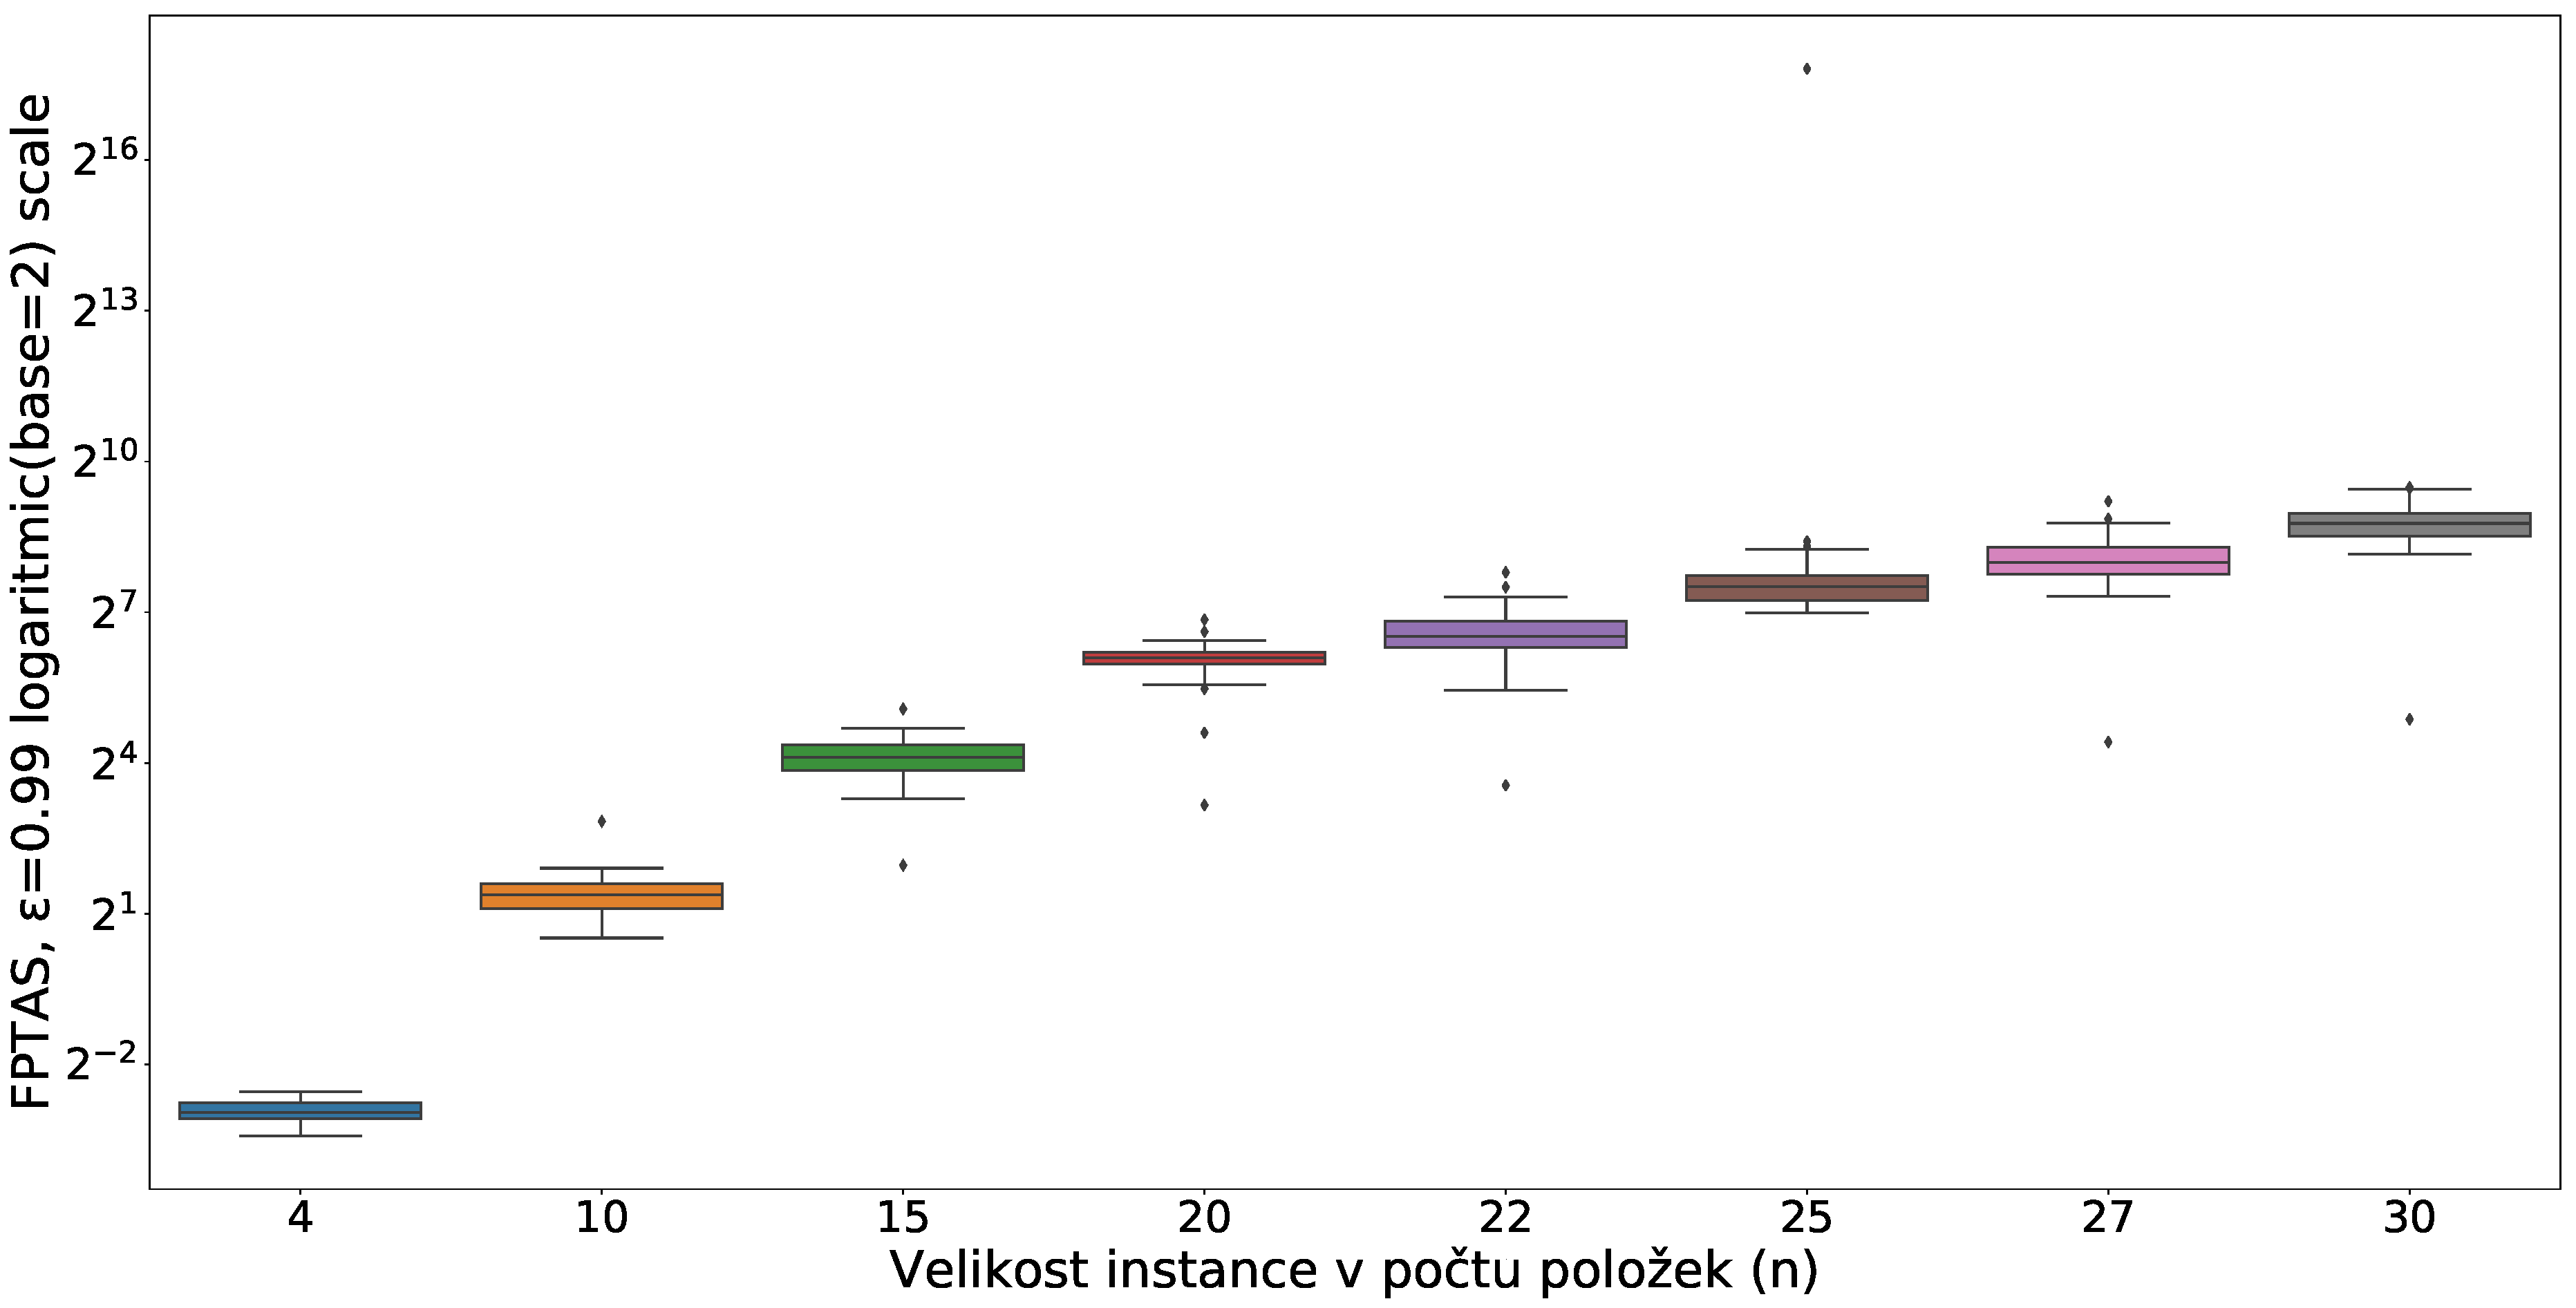
\includegraphics[scale=0.2]{img/boxF99}
 	\caption[2]{Krabicový graf popisující variabilitu měření metody FPTAS $\epsilon = 0.99$ vždy pro 50 instancí problému.}\label{fig:12}
 \end{figure} 	

Na dalším grafu jsem zobrazil závislost časové složistosti na velikosti povolené chyby. Zde jsem uvedl graf \ref{fig:13} této závisloti na velikosti instance 25. Na dalším grafu \ref{fig:14} je stejná závislost pro velikost instance 27, kde došlo k aproximování těžkých problémů pro vysoké hodnoty $\epsilon$.
 
\begin{figure}[h]\centering
	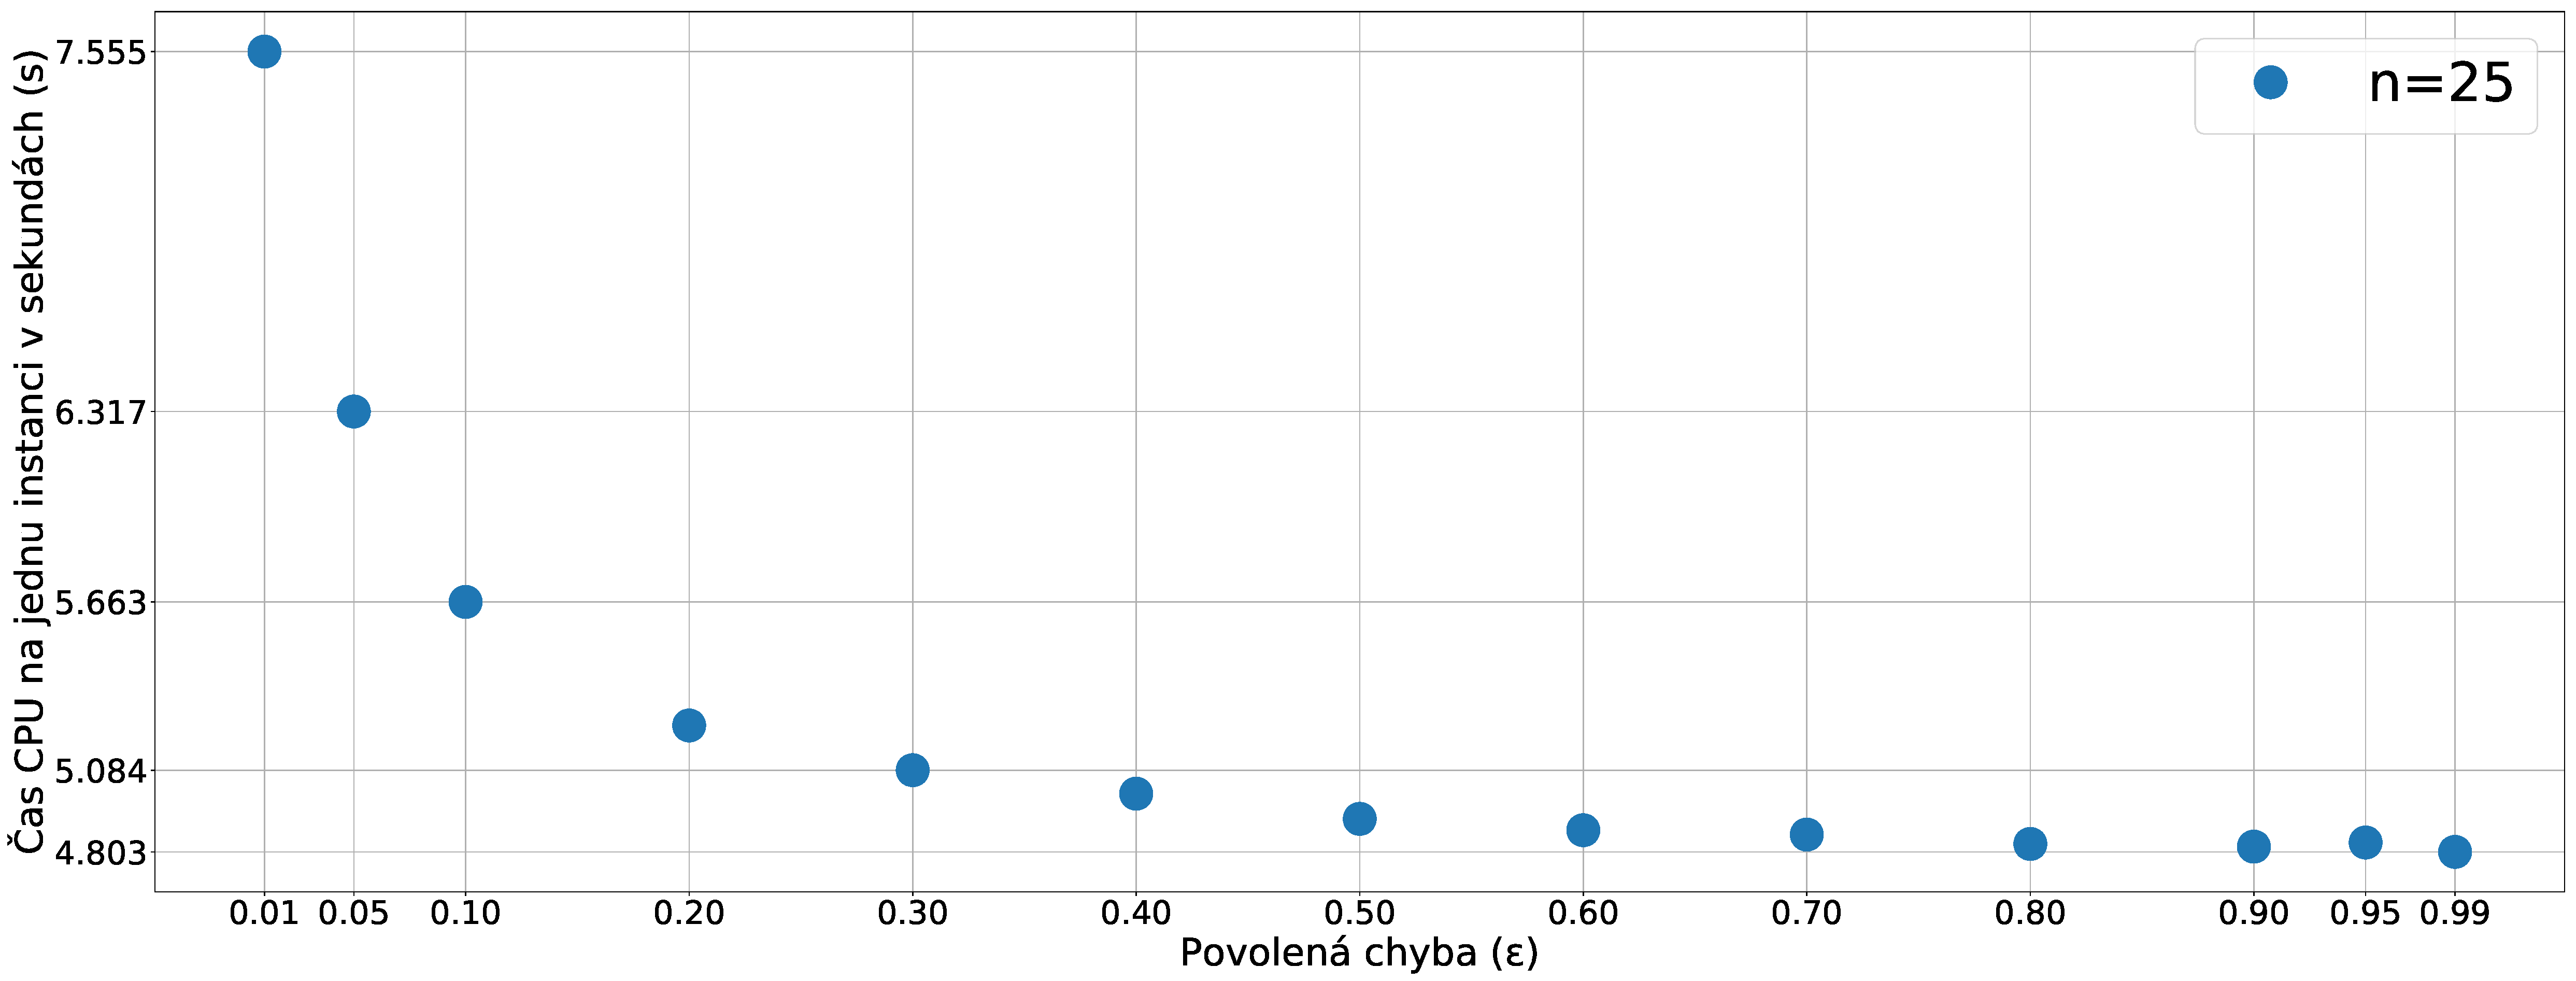
\includegraphics[scale=0.2]{img/FPTASTimeEPS25}
 	\caption[2]{Graf ukazující závislost výpočetního času a zvolené maximální chyby $\epsilon$ pro velikost instance 25.}\label{fig:13}
 \end{figure} 	
 \begin{figure}[h]\centering
	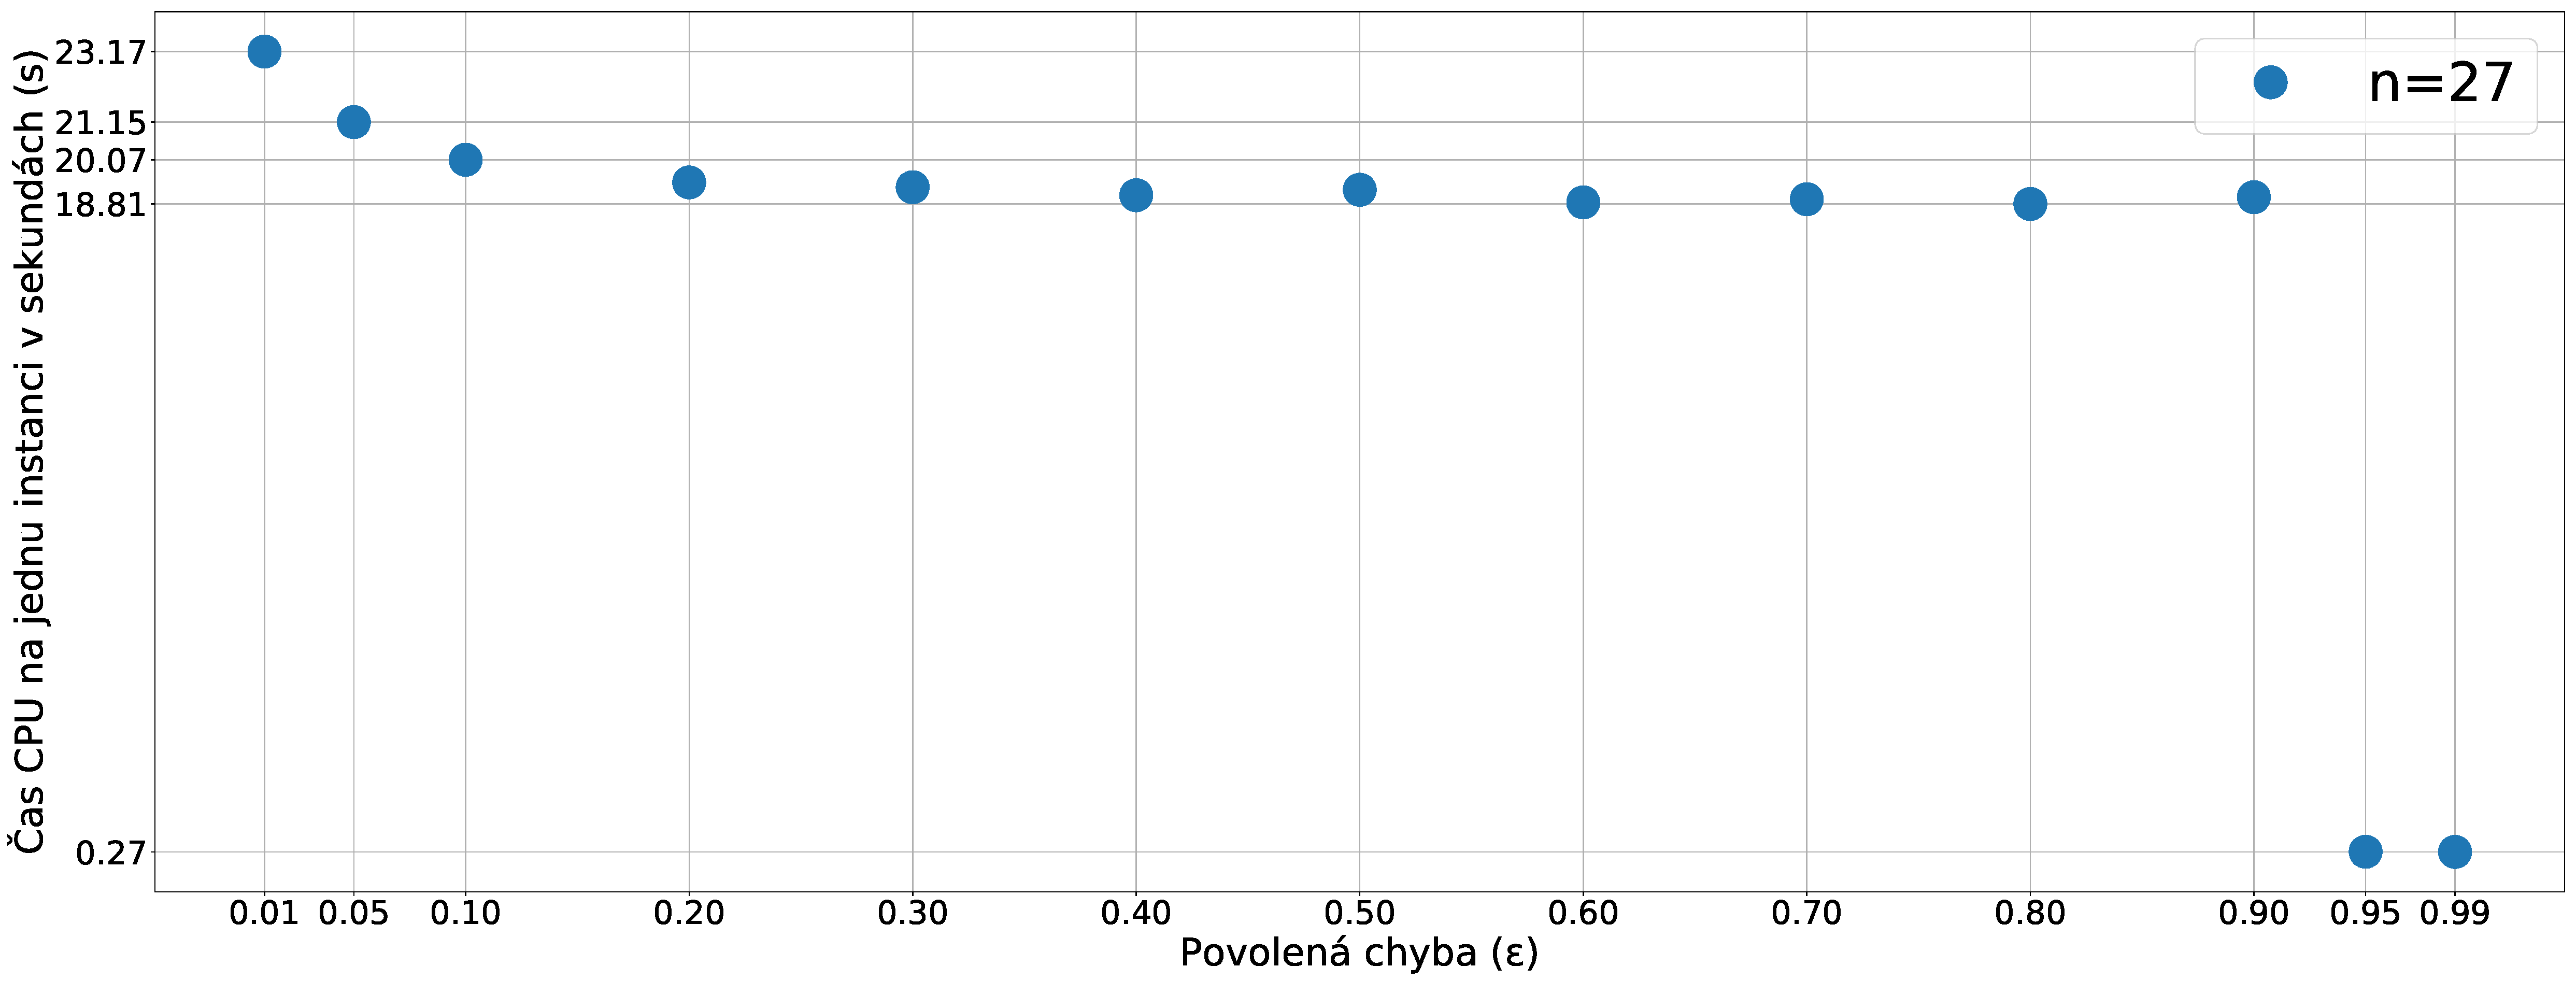
\includegraphics[scale=0.2]{img/FPTASTimeEPS27}
 	\caption[2]{Graf ukazující závislost výpočetního času a zvolené maximální chyby $\epsilon$ pro velikost instance 25.}\label{fig:14}
 \end{figure} 	 
 
\subsection{FPTAS meření relativní chyby} 
 Na grafu \ref{fig:15} je vidět závislost maximální chyby pro různě zvolenou maximální chybu v algoritmu FPTAS pro měřená n. Meřená chyba nikdy nepřekonala stanovenou maximální chybu. Na dalším grafu \ref{fig:16} je nejvyšší hodnota z grafu \ref{fig:15} dána do srovnání s heuristikou cena/hmotnost. Zde je vidět, že heuristika vykazuje vetší chybu než algoritmus FPTAS i pro zvolenou velkou maximální chybu algoritmu, která nám negarantuje témeř nic. Na posledním grafu \ref{fig:17} je vidět závislost maximální chyby na $\epsilon$ pro vybraná $n$. Je opravdu vidět, že skutečná chyba je mnohem menší než předpokládaná maximální relativní chyba.
 
 \begin{figure}[h]\centering
	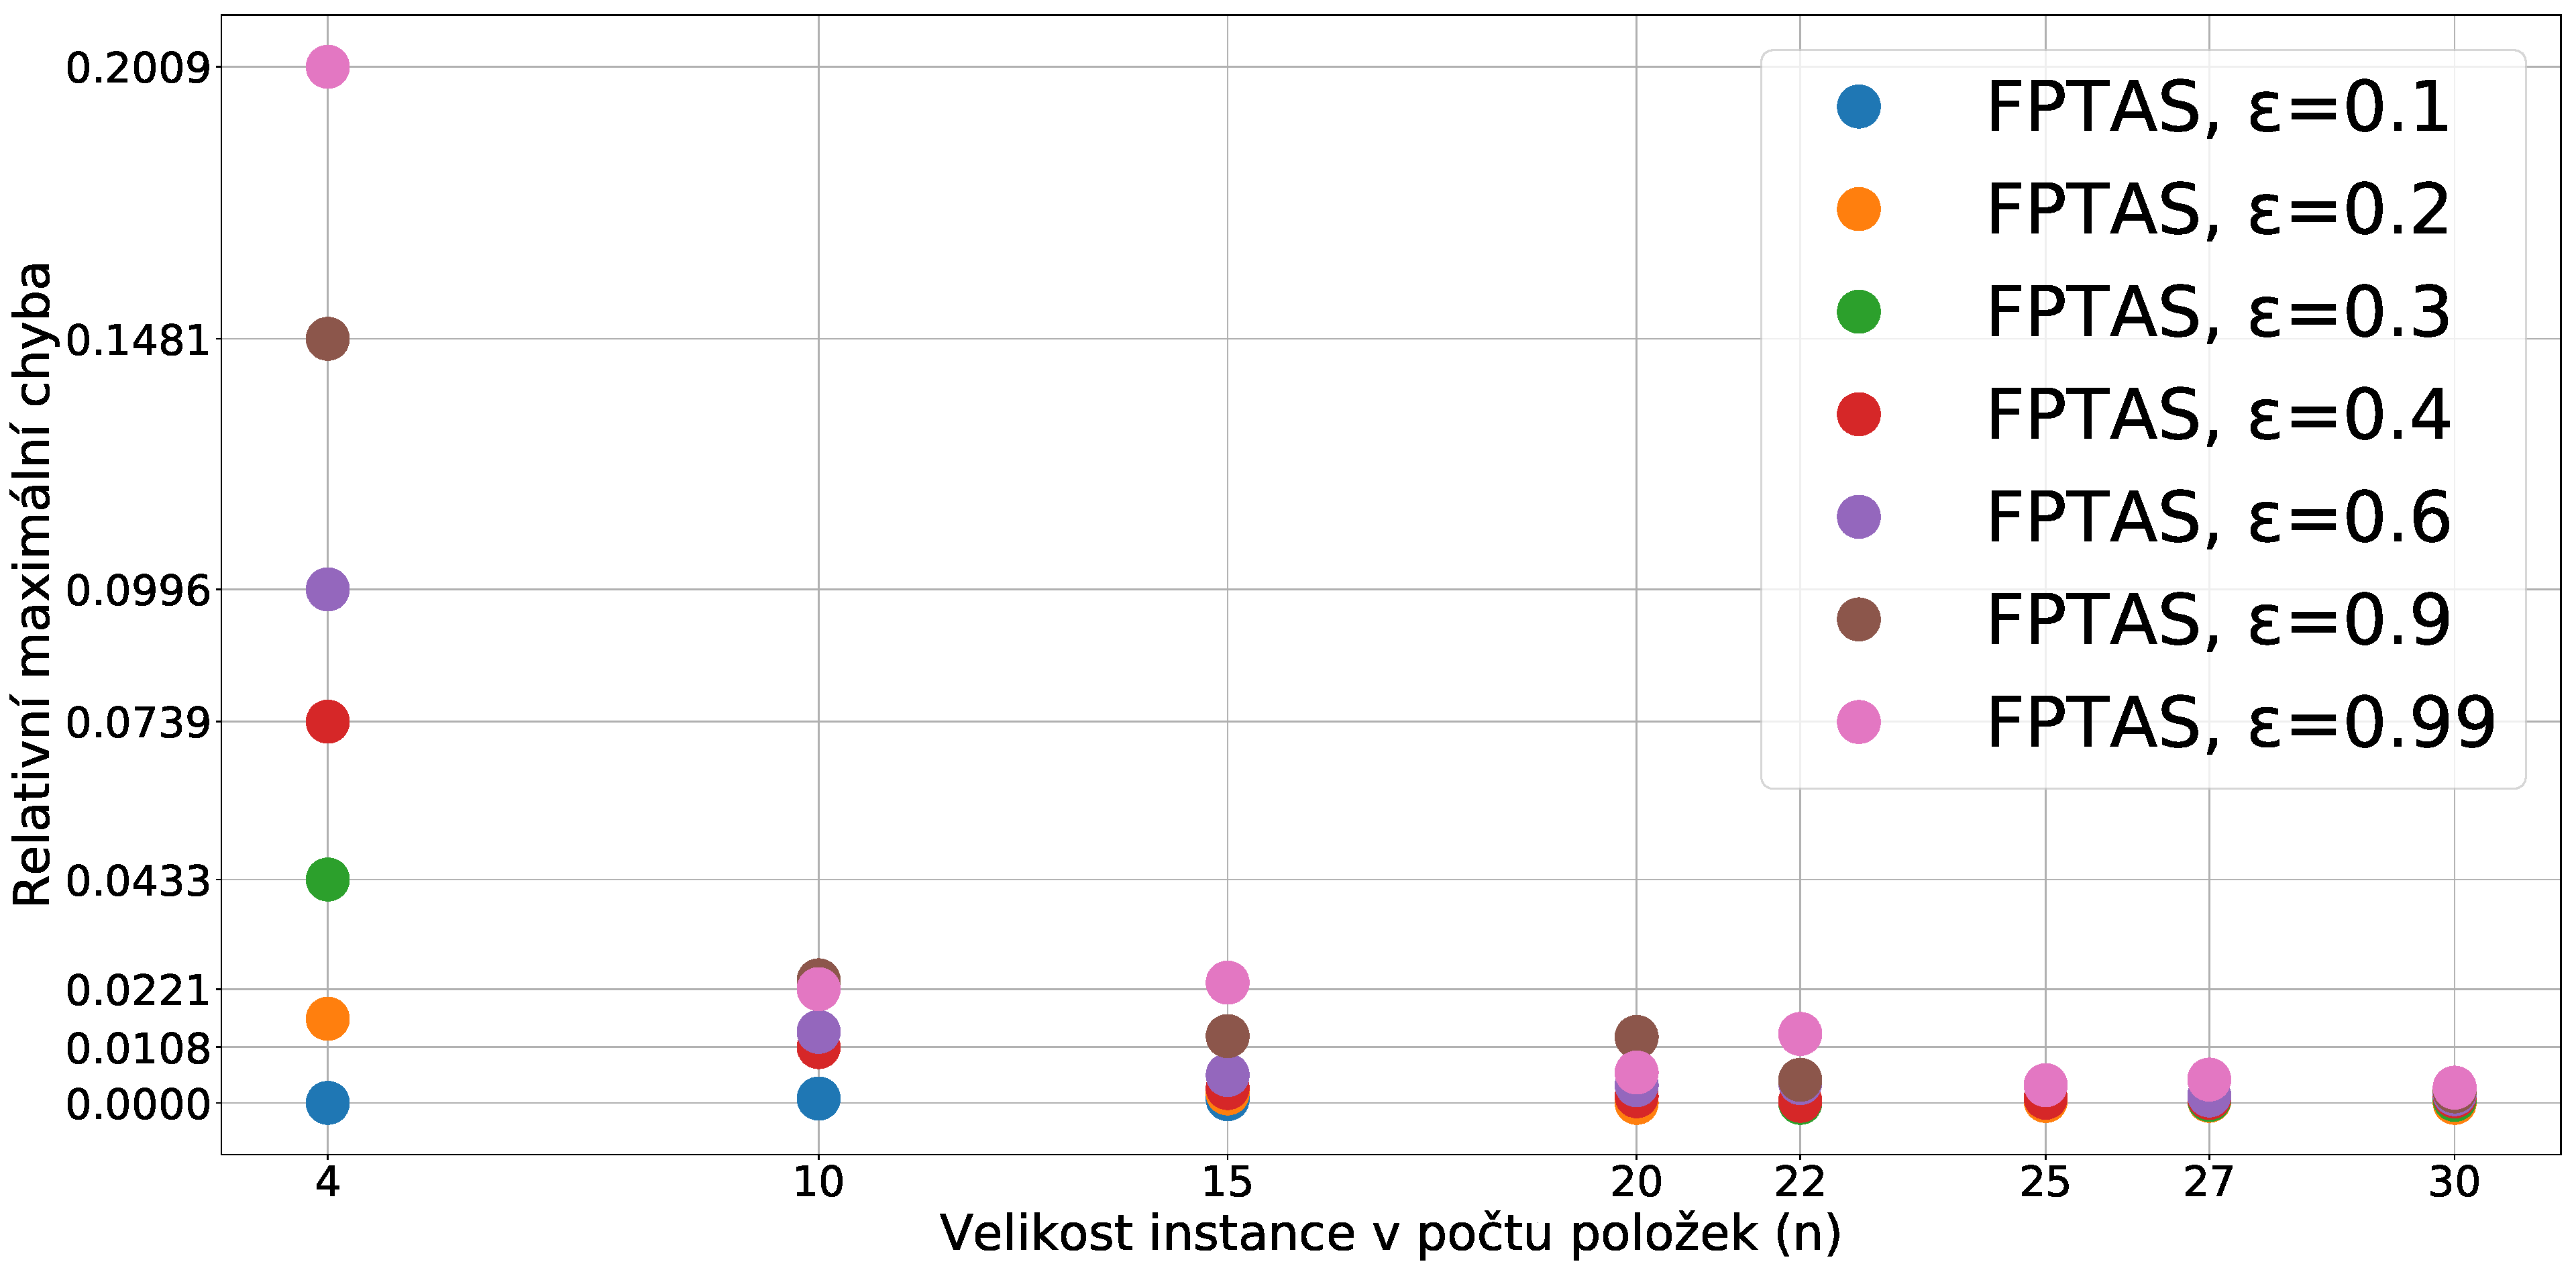
\includegraphics[scale=0.2]{img/errorFPTAS}
 	\caption[2]{Graf ukazující závislost maximální relativní chyby na velikosti instance pro několik zvolených maximálních chyb $\epsilon$.}\label{fig:15}
 \end{figure} 	
 \begin{figure}[h]\centering
	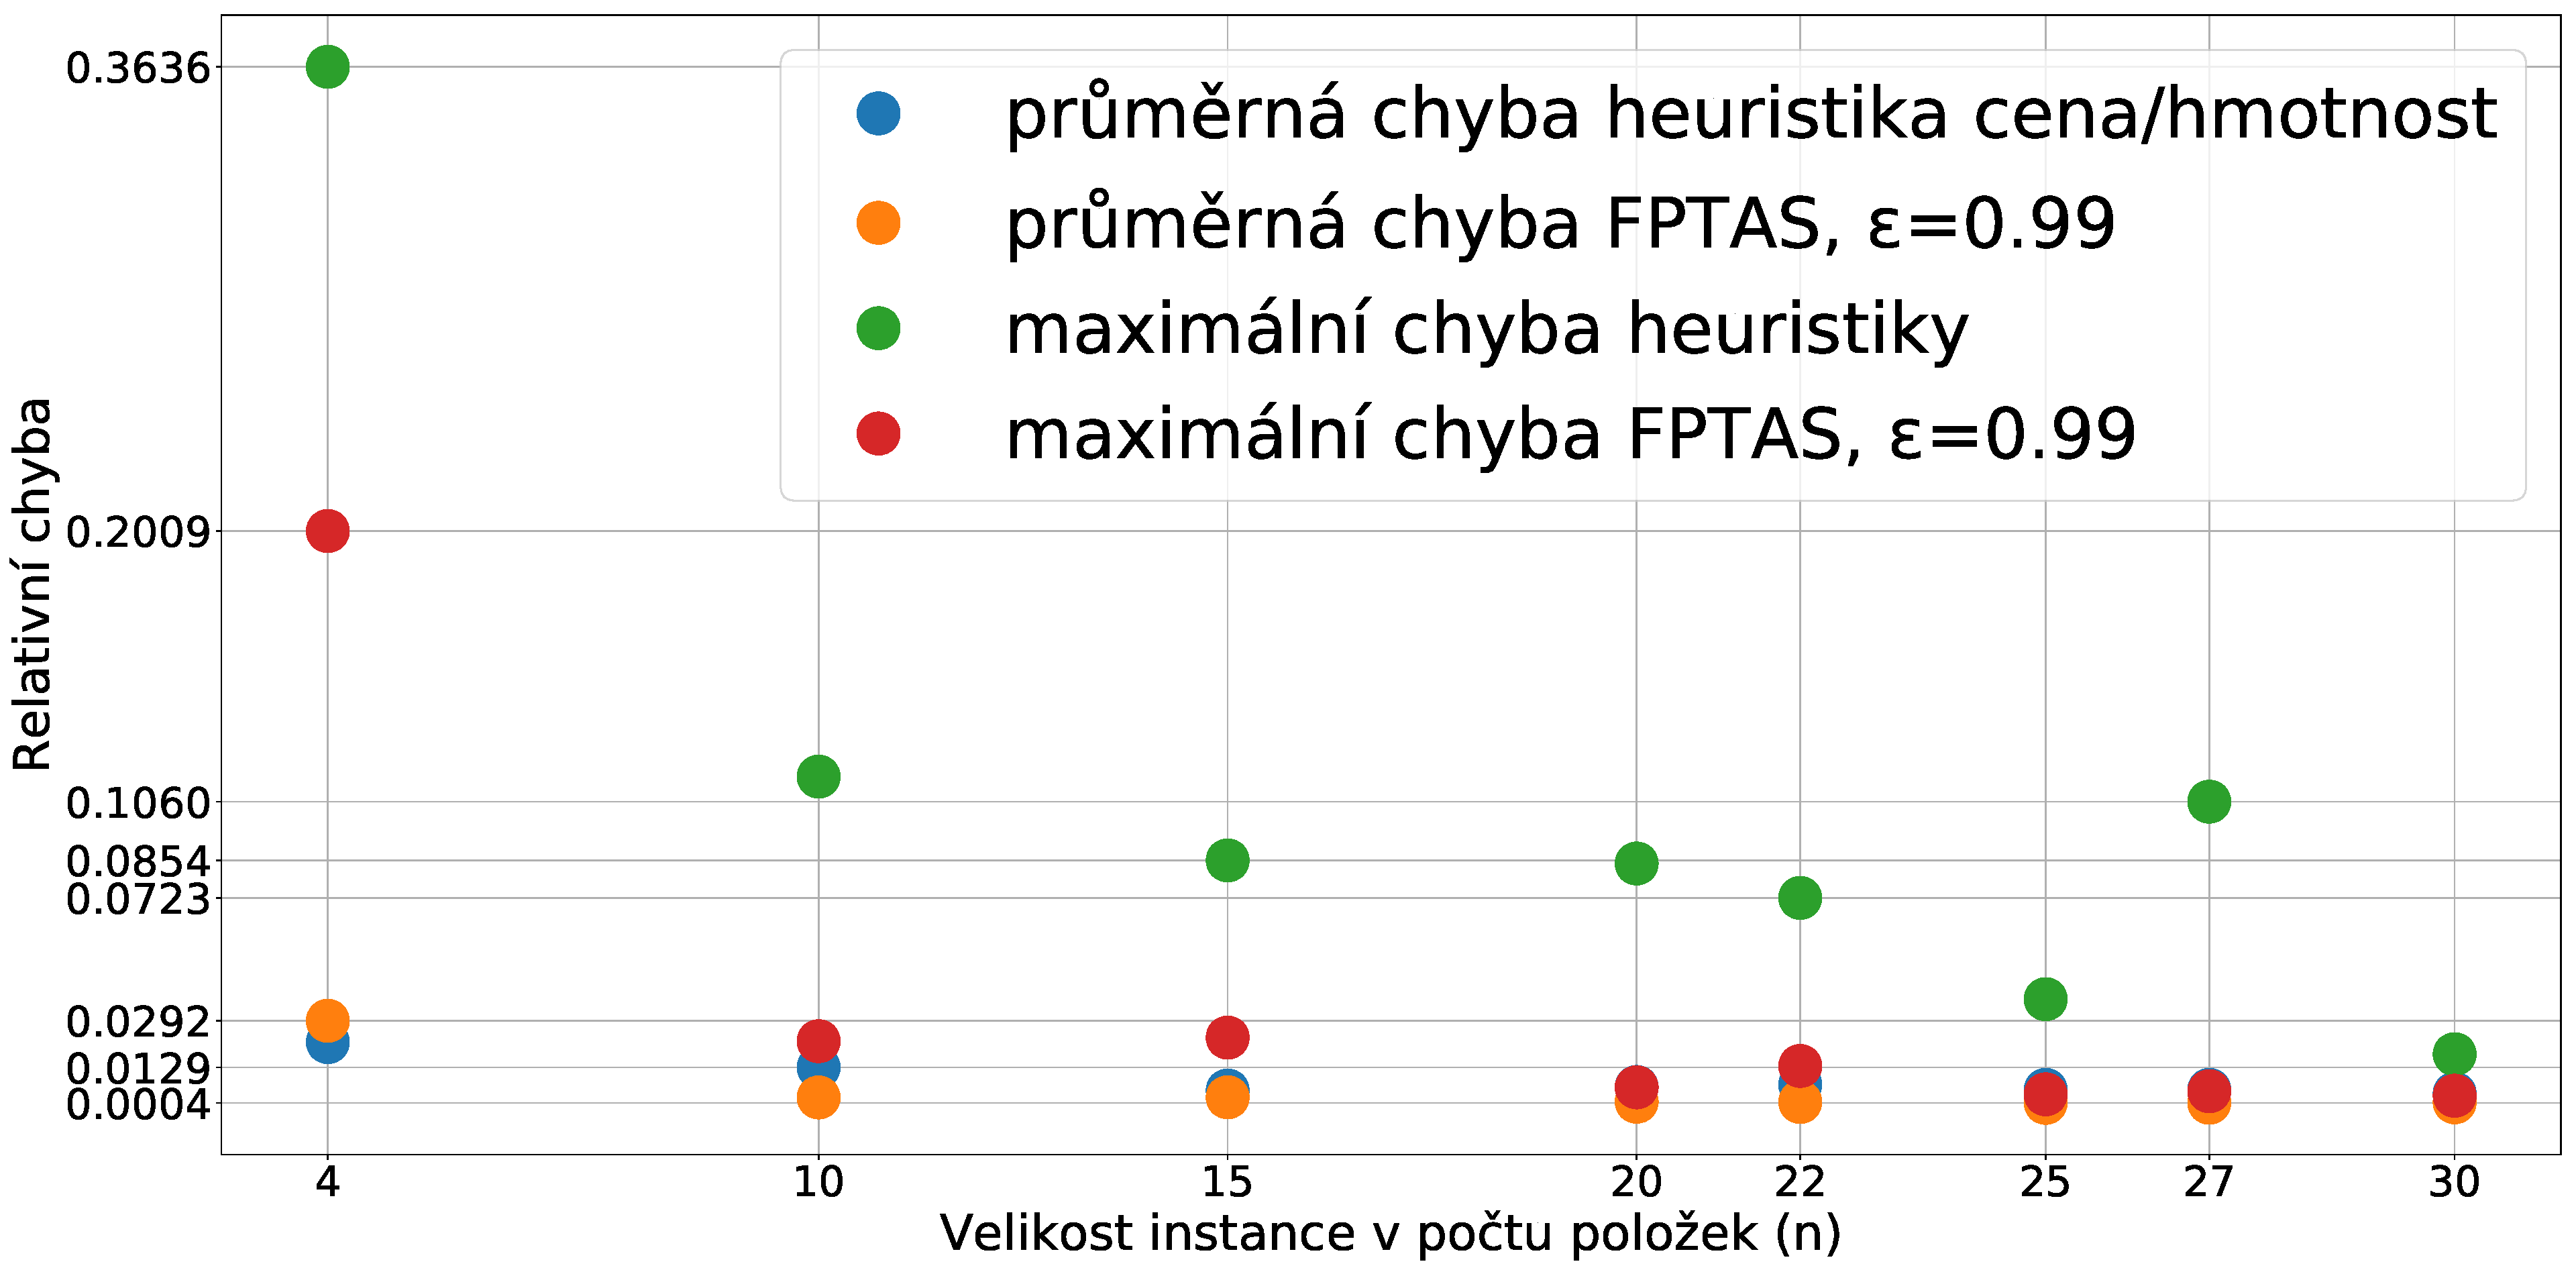
\includegraphics[scale=0.2]{img/error}
 	\caption[2]{Graf ukazující závislost maximální relativní chyby na velikosti instance pro vybranou maximální chybu ve srovnání s chybou heuristiky cena/hmotnost.}\label{fig:16}
 \end{figure} 	 
 \begin{figure}[h]\centering
	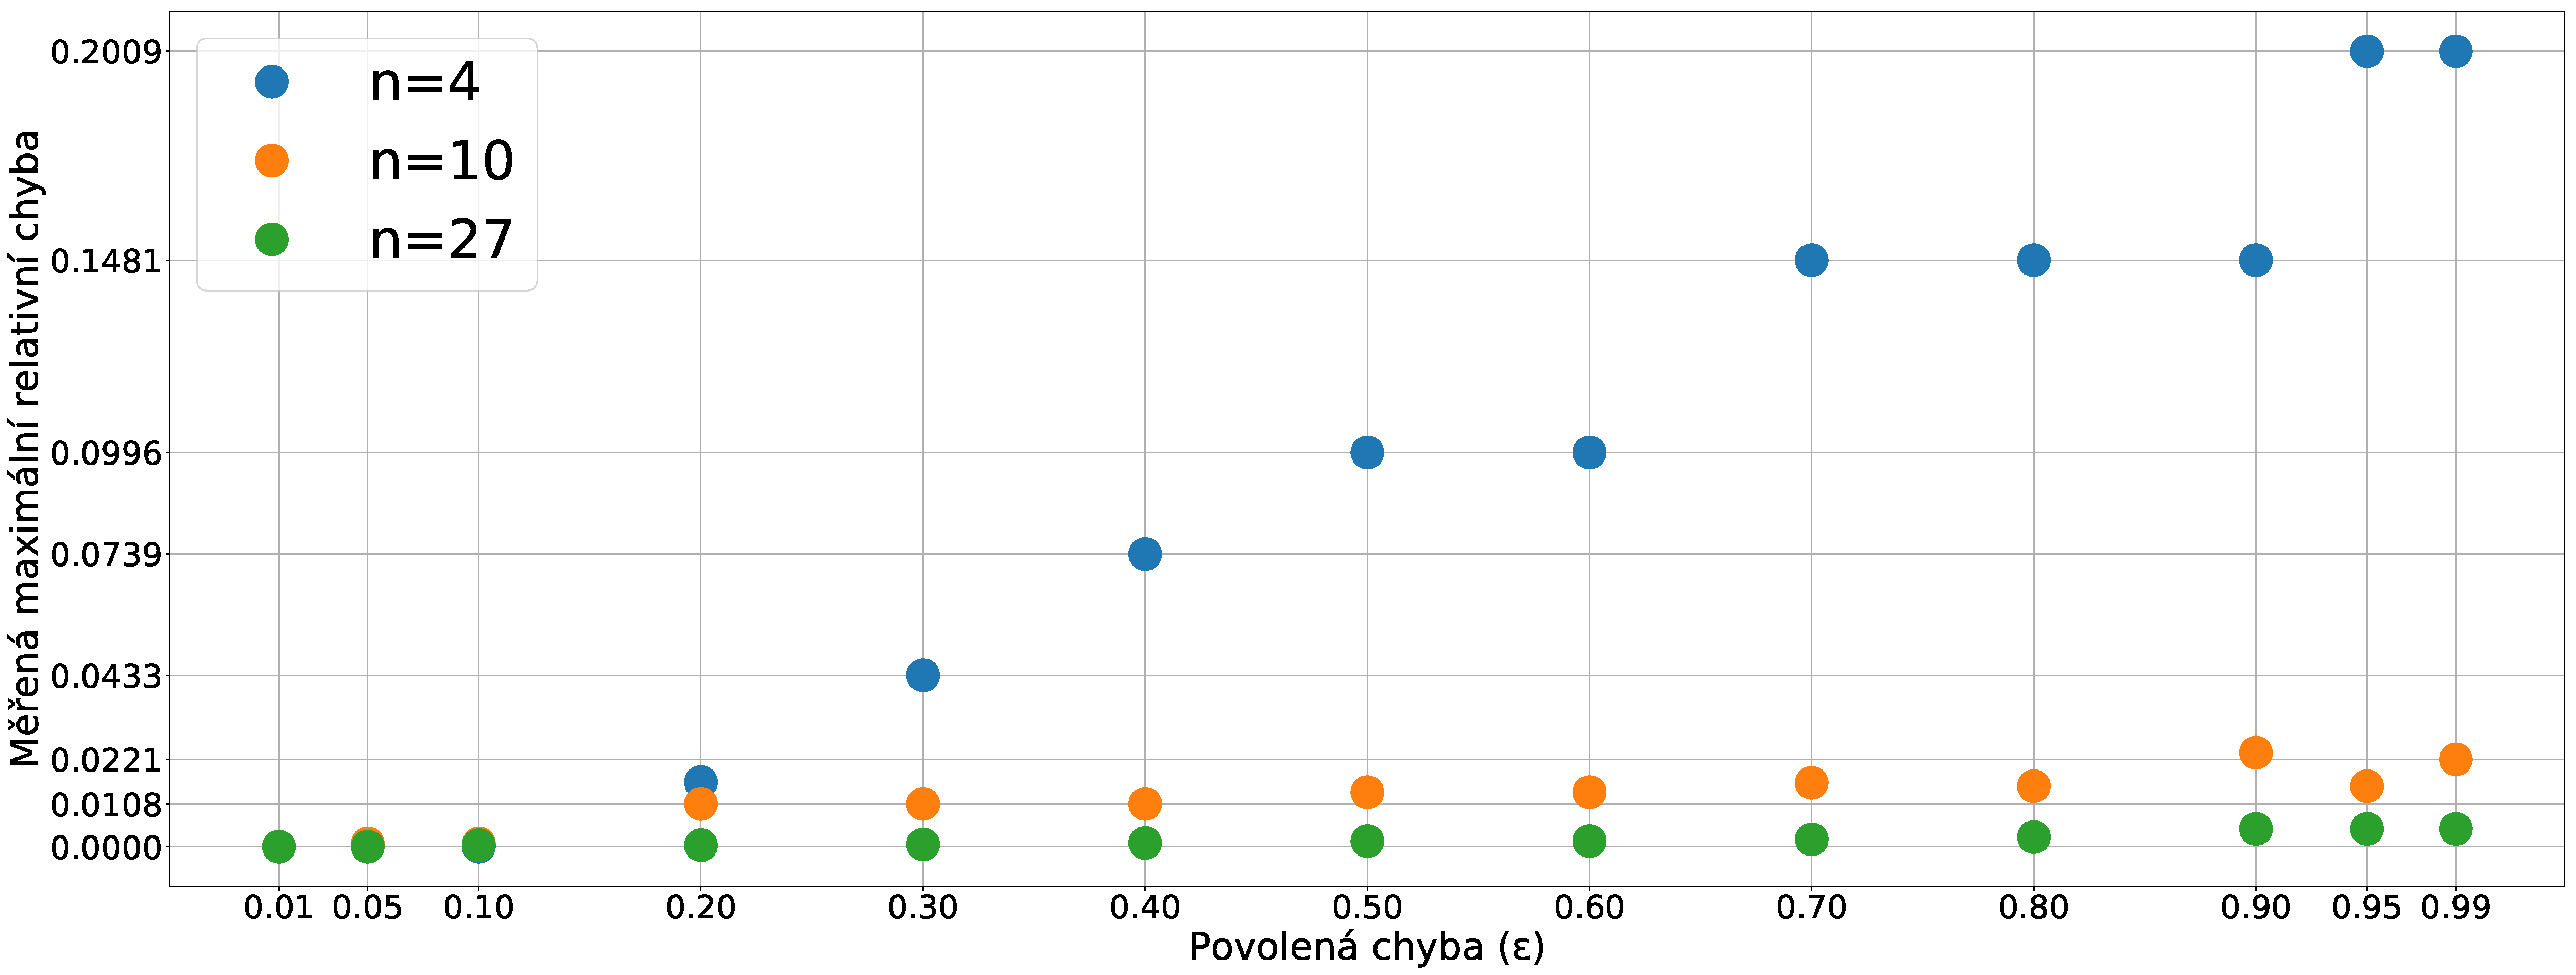
\includegraphics[scale=0.2]{img/FPTASerrEPS}
 	\caption[2]{Graf ukazující závislost relativní chyby a zvolené maximální chyby $\epsilon$ pro vybrané velikosti instance.}\label{fig:17}
 \end{figure} 	 	 
 
\section{Závěr}
Během měření se podařilo zjistit, metody B\&B a dynamického programování dosahují velkého rozdílu ve složitosti oproti metodě hrubé síly. Dále, že dekompozice podle kapacity dosahuje nižších časů než dekompozice podle ceny. Metody dynamického programování mění složitost, která již není závislá exponenciálně na počtu předmětů, ale je ovlivněna hodnotami dané instance.

 Podle měření byla z exaktních metod nejrychlejší metoda větví a hranic (měla by mít stále exponenciální složitost). Tato metoda však měla velký rozptyl meřených časů pro různé instance. Při přištích experimentech by bylo zajímavé metody dynamického programování vylepšit o metody B\&B a zkusit naměřit výsledky.

Při měření jsem také narazil na fakt, že pro testované metody existují instance, pro které trvá výpočet velmi dlouho tvz. těžké instance. Pro různé instance tedy může být optimální jiný algoritmus, který jí vyřeší rychleji nebo algoritmus, který ji vyřeší s minimální chybou.

Plně polynomiální aproximační schéma FPTAS bylo zajímávé v tom, že jsme mohli měnit maximální povolenou relativní chybu a tím ovlivňovat časovou náročnost. Proto při volbě tohoto algoritmu je důležité zvážit požadavky na chybu a na rychlost a zvolit správné nastavení.

\end{document}